%% ------------------------------------------------------------------
%% AUTO-GENERATED by FlattenGlossary.py
%% Source: /Users/junga1/AaltoDictionaryofML.github.io/ADictML_Math.tex
%% Repo root: /Users/junga1/AaltoDictionaryofML.github.io
%% ------------------------------------------------------------------

\newglossaryentry{psd}
{name={positive semi-definite (psd)},
	description={A\index{positive semi-definite (psd)} (real-valued) 
	             symmetric matrix $\mathbf{Q}= \mathbf{Q}\,^{T} \in \mathbb{R}^{d\times d}$ 
	 	         is referred to as psd if ${\bf x}\,^{T} \mathbf{Q}{\bf x}\geq 0$ 
				 for every vector ${\bf x}\in \mathbb{R}^{d}$. 
	 	         The property of being psd can be extended from matrices to (real-valued) 
	 	         symmetric kernel maps $K: \mathcal{X}\times \mathcal{X}\rightarrow \mathbb{R}$ 
	 	         (with $K({\bf x},{\bf x}') = K({\bf x}',{\bf x})$)
	 	         as follows: For any finite set of feature vectors ${\bf x}^{(1)}, \,\ldots, \,{\bf x}^{(m)}$, 
	 	         the resulting matrix $\mathbf{Q}\in \mathbb{R}^{m\times m}$ with 
		        entries $Q_{r,r'} = K\big({\bf x}^{(r)},{\bf x}^{(r')}\big)$ 
		        is psd \cite{LearningKernelsBook}.
			\\
		See also: matrix, kernel.},
	first={positive semi-definite (psd)},
	type=math, 
	text={psd}  
}

\newglossaryentry{normalmatrix}
{name={normal matrix},
	description={A square matrix ${\bf A}\in \mathbb{C}^{d\times d}$ 
                 that commutes with its conjugate transpose, i.e., ${\bf A}{\bf A}^{H}={\bf A}^{H}{\bf A}$. 
                 Normal matrices admit an orthonormal basis of eigenvectors and are 
                 unitarily diagonalizable.},
	first={normal matrix},
    type=math, 
	plural={normal matrices},
	firstplural={normal matrices},
	text={normal matrix}
}

\newglossaryentry{spectraldecomp}
{name={spectral decomposition},
	description={Every normal matrix ${\bf A}\in \mathbb{C}^{d\times d}$ 
                 admits\index{spectral decomposition} a spectral decomposition of the form \cite{HornMatAnalysis,Axler2025}
       \begin{align}
        \nonumber
            {\bf A}& = \sum_{j=1}^{d} \lambda_{j} {\bf u}^{(j)} \big({\bf u}^{(j)})^{H} \nonumber \\ 
       \end{align}
      with an orthonormal basis ${\bf u}^{(1)},\ldots,{\bf u}^{(d)}$. 
       \begin{figure}[t]
            \centering
            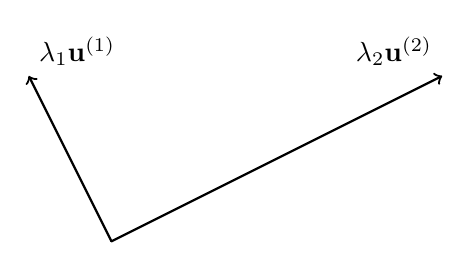
\begin{tikzpicture}[scale=2.1, line cap=round, line join=round]
            
            \draw[->, thick] (0,0) -- (-0.5,1) node[above right] {$\lambda_{1} {\bf u}^{(1)}$};
            \draw[->, thick] (0,0) -- (2.0,1) node[above left]  {$\lambda_{2} {\bf u}^{(2)}$};
            \end{tikzpicture}
            \caption{The spectral decomposition of a normal matrix ${\bf A}$ provides 
                     an orthonormal basis ${\bf u}^{(1)}, {\bf u}^{(2)}$. Applying ${\bf A}$ 
                     amounts to a scaling of the basis vectors by the 
                     eigenvalues $\lambda_{1},\lambda_{2}$.\label{fig:eigenvectors-length_dict}}
            \end{figure}
       Each basis element ${\bf u}^{(j)}$ 
       is an eigenvector of ${\bf A}$ with corresponding eigenvalue $\lambda_{j}$, 
       for $j=1,\ldots,d$.
       },
	first={spectral decomposition},
    type=math,
	text={spectral decomposition}
}


\newglossaryentry{symmetricmatrix}
{name={symmetric matrix},
	description={A square\index{symmetric matrix} matrix ${\bf A}$ with real-valued 
                 entries that is equal to its transpose, i.e., ${\bf A}={\bf A}^{T}$. Every 
                 symmetric matrix is a normal matrix.},
	first={symmetric matrix},
	plural={symmetric matrices},
    type=math,
	firstplural={symmetric matrices},
	text={symmetric matrix}
}

\newglossaryentry{transpose}
{name={transpose},
 description={The transpose\index{transpose} of a real-valued matrix is obtained by exchanging 
                  rows and columns. For a matrix ${\bf A}\in \mathbb{R}^{m\times d}$, 
				  its transpose is denoted ${\bf A}^{T}$ and satisfies $\big({\bf A}^{T}\big)_{j,j'}=\mA_{featureidx',j}$.},
 	first={transpose},
    type=math, 
 	text={transpose}
 }

 \newglossaryentry{conjugatetranspose}
{name={conjugate transpose},
 description={The conjugate transpose\index{conjugate transpose} of a 
              matrix is obtained by transposing the matrix 
			  and taking the complex conjugate of each entry.
              For a matrix ${\bf A}\in \mathbb{C}^{m\times d}$, its
              conjugate transpose is denoted by ${\bf A}^{H} \in 
              \mathbb{C}^{d\times m}$ and is defined entrywise by
              \[
                 ({\bf A}^{H})_{j,r}
                 = \overline{\big({\bf A}\big)_{r,j}},
              \]
              where $\overline{(\cdot)}$ denotes complex conjugation.},
 	first={conjugate transpose},
    type=math, 
 	text={conjugate transpose}
 }

\newglossaryentry{hermitian}
 {name={Hermitian (matrix)},
 	description={A square\index{Hermitian} matrix ${\bf A}\in \mathbb{C}^{d\times d}$ is 
	             Hermitian if it coincides with its conjugate transpose, i.e., ${\bf A}={\bf A}^{H}$. 
                 Trivally, a Hermitian matrix is also a normal matrix.},
 	first={Hermitian},
     type=math, 
 	plural={Hermitian},
 	firstplural={Hermitian},
 	text={Hermitian}
}

\newglossaryentry{dimension}
{name={dimension},
	description={The\index{dimension} dimension $\dim \mathcal{A}$ of a 
		vector space $\mathcal{A}$ is the cardinality of any 
		basis of $\mathcal{A}$ \cite{StrangLinAlg2016}. 
		Strictly speaking, this definition applies only to finite-dimensional vector spaces, 
		i.e., those that possess a finite basis. 
		\begin{figure}[H]
			\begin{tikzpicture}[scale=1]
  			
  			
  			
  			\coordinate (O) at (0,0);
  			
  			\draw[->, thick] (O) -- (1.8,0) node[below right] {${\bf e}^{(1)}$};
  			\draw[->, thick] (O) -- (0,1.6) node[above left] {${\bf e}^{(2)}$};
  			
			\draw[->, thick, dashed, shift={(3.5,0.5)}] (0,0) -- (1.2,1.2) node[above right] {${\bf u}^{(1)}$};
			\draw[->, thick, dashed, shift={(3.5,0.5)}] (0,0) -- (-1.2,1.2) node[above left] {${\bf u}^{(2)}$};
  			
  			\draw[->, thick, dotted, shift={(-2.5,-2.5)}] (O) -- (2.0,0.6) node[above right] {${\bf w}^{(1)}$};
  			\draw[->, thick, dotted, shift={(-2.5,-2.5)}] (O) -- (0.4,1.8) node[left] {${\bf w}^{(2)}$};
  			
 			
 			
			\end{tikzpicture}
		\caption{Three bases, $\big\{{\bf e}^{(1)},{\bf e}^{(2)} \big\}, \big\{{\bf u}^{(1)},{\bf u}^{(2)} \big\},
		\big\{{\bf w}^{(1)},{\bf w}^{(2)} \big\}$, for the vector space $\mathbb{R}^{2}$.} 
		\end{figure}
		For such spaces, all bases have the same cardinality, which is the dimension of the space 
		\cite[Ch.~2]{Axler2025}.	
   			 \\
		See also: vector space, basis. }, 
	text={dimension}, 
	type=math,
	first={dimension}  
}

\newglossaryentry{linearlyindep}
{name={linearly independent},
	description={A subset $\{{\bf a}^{(1)}, \,\ldots, \,{\bf a}^{(d)}\} \in \mathcal{V}$ 
		of a vector space is linearly independent\index{linearly independent} 
		if there is no nontrivial linear combination of these vectors that 
		equals the zero vector \cite{StrangLinAlg2016}. 
		In other words, $$\sum_{j=1}^{d} \alpha_{j} {\bf a}^{(j)} = \mathbf{0}	
		\quad \text{ implies } \quad \alpha_{1} = \alpha_{2} = \ldots = \alpha_{k} = 0.$$ 
			\\ 
		See also: vector space, vector, dimension, basis.}, 
	text={linearly independent}, 
	type=math,
	first={linearly independent}  
}

\newglossaryentry{basis}
{name={basis},
	description={A basis\index{basis} of a vector space $\mathcal{V}$ 
		is a set of linearly independent vectors $\{{\bf a}^{(1)}, \,\ldots, \,{\bf a}^{(d)}\}$ such 
		that any vector ${\bf a}\in \mathcal{A}$ can be expressed as a linear combination 
		of the basis vectors, i.e.,	
		$$ {\bf a}= \sum_{j=1}^{d} \alpha_{j} {\bf a}^{(j)} 
		\quad \text{ for some } \alpha_{1}, \,\ldots, \,\alpha_{d} \in \mathbb{R}. $$
			\\
		See also: vector space, linearly independent, vector. },
	text={basis}, 
	firstplural={bases}, 
	plural={bases}, 
	type=math,
	first={basis} 
}


\newglossaryentry{widematrix}
{name={wide matrix},
 description={A\index{wide matrix} matrix 
   		${\bf X}\in \mathbb{R}^{m\times d}$ 
		is referred to as wide if it has more columns than rows, 
		i.e., when $d> m$.
		\begin{figure}[H]
			\centering
			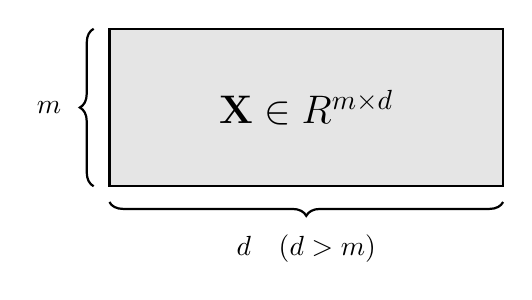
\begin{tikzpicture}
				\def\matHeight{2}
				\def\matWidth{5} 
				\draw[thick, fill=gray!20] (0,0) rectangle (\matWidth, \matHeight);
				\node at (0.5*\matWidth, 0.5*\matHeight) {\Large ${\bf X}\in \mathbb{R}^{m\times d}$};
				
				\draw[decorate, decoration={brace, amplitude=5pt}, thick] 
  					(-0.2, 0) -- (-0.2, \matHeight)
  					node[midway, left=8pt] {$m$};
				\draw[decorate, decoration={brace, amplitude=5pt, mirror}, thick] 
        			(0, -0.2) -- (\matWidth, -0.2) 
        			node[midway, below=8pt] {$d\quad (d> m)$};
			\end{tikzpicture}
		\end{figure}
		See also: matrix. },
	text={wide matrix}, 
	firstplural={wide matrices}, 
	plural={wide matrices}, 
	type=math,
   	first={wide matrix} 
}

\newglossaryentry{randomexperiment}
{name={random experiment},
	description={A random experiment\index{random experiment} is a physical (or abstract) process 
    	 	that produces an outcome $\omega$ from a set $\Omega$ of possibilities. 
	 	This set of all possible outcomes is referred to as the sample space of 
	 	the experiment. The key characteristic of a random experiment is that its 
	 	outcome is unpredictable (or uncertain). Any measurement or observation 
	 	of the outcome is a random variable (RV), i.e., a function of the outcome $\omega\in \Omega$. 
	 	Probability theory uses a probability space as a mathematical structure for the study of 
	 	random experiments. A key conceptual property of a random experiment is that it can 
	 	be repeated under identical conditions. Strictly speaking, repeating a random experiment 
	 	a given number of $m$ times defines a new random experiment. The outcomes 
	 	of this new experiment are length-$m$ sequences of outcomes 
	 	from the original experiment (see Fig. \ref{fig_randomexperiment_dict}). While the outcome of a single experiment is 
	 	uncertain, the long-run behaviour of the outcomes of repeated experiments 
	 	tends to become increasingly predictable. This informal claim can be made 
	 	precise via fundamental results of probability theory, such as the law of large numbers 
	 	and the central limit theorem (CLT).
	 	\begin{figure}[H]
		\begin{center}
	 		\begin{tikzpicture}[>=Stealth, node distance=1.5cm and 2cm, every node/.style={font=\small}]
			\node (experiment) [draw, rectangle, rounded corners, minimum width=2.6cm, align=center] {random\\experiment};
			\node (omega) [right=of experiment] {$\omega\in \Omega$};
			\coordinate (rightpad) at ($(omega.east) + (0.2,0)$);
			\draw[->] (experiment) -- (omega);
			\node (sequence) [below=of experiment, yshift=-0.5cm] {$(\omega^{(1)}, \,\omega^{(2)}, \,\dots, \,\omega^{(m)})$};
			\node (sequence1) [below=of sequence, yshift=-0.5cm] {$({\bf z}^{(1)}, \,{\bf z}^{(2)}, \,\dots, \,{\bf z}^{(m)})$};
			\draw[->, thick] (experiment.south) -- node[midway, right, xshift=3pt] {repeat $m$ times} (sequence.north);
			\draw[->, thick] (sequence.south) -- node[midway, right, xshift=3pt] {random variables (RVs)} (sequence1.north);
			
			\path (experiment.south) -- (sequence.north) coordinate[pos=0.6] (repeatpoint);
			
        			\node[draw=black, rounded corners, dotted, fit={(experiment) (repeatpoint) (rightpad)}, inner sep=8pt, label=above:{new random experiment with $\Omega' = \Omega\times \ldots \times \Omega$}] {};
	 		\end{tikzpicture}
	     	\end{center}
		\caption{A random experiment produces an outcome $\omega\in \Omega$ from a set 
		of possibilities (i.e., a sample space) 
		$\Omega$. Repeating the experiment $m$ times yields another random 
		experiment, whose outcomes are sequences 
		$(\omega^{(1)}, \,\omega^{(2)}, \,\dots, \,\omega^{(m)}) \in \Omega\times\ldots\times \Omega$. 
		One example of a random experiment arising in many machine learning (ML) applications is the gathering 
		of a training set ${\bf z}^{(1)},\,\ldots,\,{\bf z}^{(m)}$. \label{fig_randomexperiment_dict}}
	 	\end{figure} 
	 	Examples for random experiments arising in machine learning (ML) applications include the following: 
	 	\begin{itemize} 
			\item Data collection: The data points collected in empirical risk minimization (ERM)-based methods 
			can be interpreted as random variables (RVs), i.e., as functions of the outcome $\omega\in \Omega$ 
			of a random experiment. 
			\item Stochastic gradient descent (SGD) uses a random experiment at each iteration to select a subset of 
			the training set. 
			\item Privacy protection methods use random experiments to perturb  
			the outputs of an machine learning (ML) method to ensure DP. 
	 	\end{itemize} 
		See also: sample space, random variable (RV), probability, probability space.},
 	firstplural={random experiments},
 	plural={random experiments},
	type=math, 
 	first={random experiment},
 	text={random experiment}
}

\newglossaryentry{pseudoinverse}
{name={pseudoinverse},
  description={The \index{pseudoinverse}Moore–Penrose pseudoinverse ${\bf A}^{+}$ 
 	of a matrix ${\bf X}\in \mathbb{R}^{m\times d}$ 
	generalizes the notion of an inverse matrix \cite{GolubVanLoanBook}. 
	The pseudoinverse arises naturally in ridge regression for a 
	dataset with feature matrix ${\bf X}$ and label vector 
	${\bf y}$ \cite[Ch.\ 3]{hastie01statisticallearning}. 
	The model parameters learned by ridge regression 
  	are given by
  	\[
  	\widehat{{\bf w}}^{(\alpha)}  = \big({\bf X}^{T} {\bf X}+ \alpha\mathbf{I}\big)^{-1} {\bf X}^{T} {\bf y}, \quad \alpha> 0.
  	\]
  	We can then define the pseudoinverse ${\bf X}^{+} \in \mathbb{R}^{d\times m}$ via 
  	the limit \cite[Ch. 3]{benisrael2003generalized}
  	\[
  	\lim_{\alpha\to 0^+} \widehat{{\bf w}}^{(\alpha)} = {\bf X}^+ {\bf y}.
  	\]
	\\
	See also: matrix, inverse matrix, ridge regression. },
 first={pseudoinverse},
 type=math, 
 text={pseudoinverse}
} 


\newglossaryentry{tallmatrix}
{name={tall matrix},
 description={A\index{tall matrix} matrix ${\bf X}\in \mathbb{R}^{m\times d}$ 
			  is referred to as tall if it has more rows than columns, i.e., 
			  when $m> d$.
			  \begin{figure}[H]
			\centering
			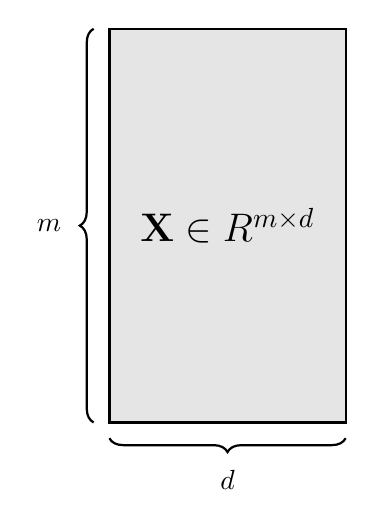
\begin{tikzpicture}
				\def\matHeight{5}
				\def\matWidth{3} 
				\draw[thick, fill=gray!20] (0,0) rectangle (\matWidth, \matHeight);
				\node at (0.5*\matWidth, 0.5*\matHeight) {\Large ${\bf X}\in \mathbb{R}^{m\times d}$};
				
				\draw[decorate, decoration={brace, amplitude=5pt}, thick] 
  					(-0.2, 0) -- (-0.2, \matHeight)
  					node[midway, left=8pt] {$m$};
				\draw[decorate, decoration={brace, amplitude=5pt, mirror}, thick] 
        			(0, -0.2) -- (\matWidth, -0.2) 
        			node[midway, below=8pt] {$d$};
			\end{tikzpicture}
		\end{figure}
		See also: matrix. },
	text={tall matrix}, 
	firstplural={tall matrices}, 
	plural={tall matrices}, 
	type=math,
   	first={tall matrix} 
}

\newglossaryentry{mgf}
{name={moment generating function (MGF)}, 
 description={Consider the\index{moment generating function (MGF)} MGF $M_{x}\left(t\right)$ 
	 	of a real-valued random variable (RV) $x$, which is defined as
	 	$M_{x}\left(t\right) = \mathbb{E} \{ \exp(t \cdot x) \}$ for any $t \in \mathbb{R}$ 
	 	for which this expectation exists \cite[Sec. 21]{BillingsleyProbMeasure}. 
		As its name indicates, the MGF allows us to compute the moments 
	 	$\mathbb{E} \{ x^{k} \}$ for $k \in \mathbb{N}$. 
	 	In particular, the $k$th moment is obtained by evaluating the $k$th 
	 	derivative of $M_{x}\left(t\right)$ for $t=0$, i.e., $\mathbb{E} \{ x^{k} \} = M_{x}^{(k)}\left(0\right)$. 
	 	This fact can be verified by the following identities: 
	 	\begin{align}
			M_{x}\left(t\right) & =\mathbb{E} \{ \exp(t \cdot x)  \} \nonumber \\ 
			& \stackrel{(a)}{=} \mathbb{E} \!\bigg\{\sum_{k=0}^{\infty} \frac{t^{k}}{k!} x^{k}\bigg\}  \nonumber \\ 
			& \stackrel{(b)}{=}  \sum_{k=0}^{\infty} \frac{t^{k}}{k!}\, \mathbb{E} \!\big\{ x^{k} \big\}. \nonumber
	 	\end{align}
	 	Here, step $(a)$ is due to the Taylor series expansion of 
	 	$\exp\,(t \cdot x)$ and step $(b)$ is valid when the MGF exists 
	 	for all $t$ in some interval $(-t_{0},t_{0})$ \cite[p. 278]{BillingsleyProbMeasure}.
	 	\begin{figure}[H]
			\centering
			\begin{tikzpicture}
			\begin{axis}[
				width=9cm, height=4.2cm,
				domain=-1:1,
				samples=200,
				
				xlabel={$x$},
				ylabel={},
				ytick=\empty,
				ytick={-1,-0.5,0,0.5,1}, 
            			yticklabels={$-1$,$-0.5$,$0$,$0.5$,$1$},
				xtick={-1,-0.5,0,0.5,1}, 
            			xticklabels={$-1$,$-0.5$,$0$,$0.5$,$1$},
				xmin=-1, xmax=1,
				legend style={at={(1.5,0.02)},anchor=south east}
				]
				
				\addplot[thick, dashed] {x};
				\addlegendentry{$x$}
				
				\addplot[thick, dotted] {x^2};
				\addlegendentry{$x^{2}$}
				
				\addplot[thick, dashdotdotted] {x^3};
				\addlegendentry{$x^{3}$}
			\end{axis}
			\end{tikzpicture}
		\caption{The first few powers of an random variable (RV) $x$. The MGF 
		encodes the moments of $x$, which are the expectations 
		of the powers $x^{k}$ for $k=1,\,2,\,\ldots$.}
		\end{figure}
		The MGF is a useful tool for the study of sums of independent 
		random variables (RVs). As a case in point, if $x$ and $y$ are independent 
		random variables (RVs), then the MGF of their sum $z = x + y$ typically 
		satisfies $M_{z}\left(t\right) = M_{x}\left(t\right)\,M_{y}\left(t\right)$,
        		i.e., the MGF of the sum is typically the pointwise product of the 
		individual MGFs \cite[p.~280]{BillingsleyProbMeasure}.
		\\
 		See also: random variable (RV), expectation. }, 
 	first={moment generating function (MGF)}, 
 	firstplural={moment generating functions (MGFs)}, 
 	plural={MGFs}, 
 	type=math, 
 	text={MGF}
} 

\newglossaryentry{chernoffbound}
{name={Chernoff bound}, 
	description={TBC\index{Chernoff bound}.}, 
 	first={Chernoff bound}, 
 	type=math, 
 	text={Chernoff bound}
}

\newglossaryentry{rankdeficient}
{name={rank-deficient},
	description={A matrix ${\bf A}\in \mathbb{R}^{m\times d}$ 
         	is rank-deficient\index{rank-deficient} if it is not full-rank, i.e., 
         	when $\rank{{\bf A}} < \min\{m,d\}$.
 		\begin{figure}[H]
			\begin{center}
			\begin{tikzpicture}[x=2cm]
				
				\begin{scope}
					\draw[->, thick] (0,0) -- (1,0) node[below] {${\bf u}^{(1)}$};
					\draw[->, thick] (0,0) -- (0,1) node[above] {${\bf u}^{(2)}$};
					
					
					
				\end{scope}
				
				\begin{scope}[shift={(3.2,0)}]
				
				
					\coordinate (A) at (0.2,0.0);
					\coordinate (B) at (2.0,0.0);
					\draw[->, very thick, red] (0,0) -- (A) node[below,yshift=-2pt] {${\bf A}{\bf u}^{(1)}$};
					\draw[->, very thick, red] (0,0) -- (B) node[above,yshift=2pt] {${\bf A}{\bf u}^{(2)}$};
					
					
				\end{scope}
				
				\draw[->, thick] (1.6,0.5) to[bend left] node[midway, above] {${\bf A}$} (2.7,0.5);
				
			\end{tikzpicture}
			\end{center}
		\caption{Example of a rank-deficient matrix 
		${\bf A}\in \mathbb{R}^{2 \times 2}$.	\label{fig_matrix_rank_defdict}} 
		\end{figure} 
		In linear regression, the solution of the empirical risk minimization (ERM) problem is not 
		unique whenever the feature matrix ${\bf X}$ is such that 
		the matrix ${\bf X}^{\top}{\bf X}$ is rank-deficient.
		\\
   		See also: full-rank, dimension, vector space. }, 
	first={rank-deficient}, 
   	type=math,
   	text={rank-deficient}
}

\newglossaryentry{fullrank}
 {name={full-rank},
 	description={A matrix ${\bf A}\in \mathbb{R}^{m\times d}$ 
  		is\index{full-rank} full-rank if it has maximum rank \cite{StrangLinAlg2016}. 
  		For a tall matrix, i.e., when $d< m$, being 
  		full-rank means that its rank is equal to $d$. 
 		\begin{figure}[H]
			\centering
			\begin{tikzpicture}[every node/.style={font=\small}]
			
			\node at (0,2) {$
			{\bf A}=
			\begin{pmatrix}
			1 & 2\\
			3 & 4
			\end{pmatrix}
			$};
			\node[below=0.8cm of {$(0,2)$}] {\small full-rank square};
			
			\node at (4.5,2) {$
			{\bf B}=
			\begin{pmatrix}
			1 & 2\\
			2 & 4
			\end{pmatrix}
			$};
			\node[below=0.8cm of {$(4.5,2)$}] {\small rank-deficient square};
			
			\node at (0,-1.0) {$
			{\bf C}=
			\begin{pmatrix}
			1 & 0\\
			0 & 1\\
			1 & 1
			\end{pmatrix}
			$};
			\node[below=1.2cm of {$(0,-1.0)$}] {\small full-rank tall matrix};
			
			\node at (4.5,-1.0) {$
			{\bf D}=
			\begin{pmatrix}
			1 & 2 & 3\\
			2 & 4 & 6
			\end{pmatrix}
			$};
			\node[below=1.2cm of {$(4.5,-1.0)$}] {\small rank-deficient wide matrix};
			\end{tikzpicture}
		\caption{Examples of full-rank and rank-deficient matrices.}
		\end{figure} 
  		A square matrix is full-rank if and only if it is invertible. 
		\\ 
  		See also: matrix, dimension, linear map, column space.}, 
	text = {full-rank}, 
  	type=math,
  	first={full-rank} 
 }

\newglossaryentry{rank}
{name={rank},
	description={The rank\index{rank} of a matrix ${\bf A}\in \mathbb{R}^{m\times d}$, 
 		denoted as $\rank{{\bf A}}$, is the maximum number of linearly independent columns 
 		of ${\bf A}$ \cite{StrangLinAlg2016}. Equivalently, the rank can be defined as the 
 		dimension of the column space ${\rm span}\left({\bf A}\right) = \big\{ {\bf A}{\bf w}\mbox{ for some } 
 		{\bf w}\in \mathbb{R}^{d} \big\}$. The rank of a matrix 
 		${\bf A}\in \mathbb{R}^{m\times d}$ can neither exceed the 
 		number of rows nor the number of columns of ${\bf A}$ \cite{Horn91}, \cite{MeyerMatrixAnalysis}, 
		i.e., $\rank{{\bf A}} \leq \min \{ m, d\}$.  
		\\ 
 		See also: matrix, dimension, column space, linear map.}, 
	text={rank}, 
	type=math,
	first={rank} 
}

\newglossaryentry{inverse}
{name={inverse matrix},
 description={An inverse matrix\index{inverse matrix} ${\bf A}^{-1}$ is defined for a 
 	square matrix ${\bf A}\in \mathbb{R}^{n \times n}$ that is of full rank, meaning its 
 	columns are linearly independent. In this case, ${\bf A}$ is said to be invertible, 
 	and its inverse satisfies 
 	\[
 	{\bf A}{\bf A}^{-1} = {\bf A}^{-1} {\bf A}= \mathbf{I}.
 	\]  	
     	A square matrix is invertible if and only if its determinant is non-zero. Inverse matrices are 
     	fundamental in solving systems of linear equations and in the closed-form solution of 
     	linear regression \cite{Strang2007}, \cite{Horn91}.  The concept of an inverse matrix can be extended 
     	to matrices that are not square or does not have full rank. One may define a ``left inverse'' ${\bf B}$ 
     	satisfying ${\bf B}{\bf A}= \mathbf{I}$ or a ``right inverse'' ${\bf C}$ satisfying ${\bf A}{\bf C}= \mathbf{I}$. 
     	For general rectangular or singular matrices, the Moore–Penrose pseudoinverse
     	${\bf A}^{+}$ provides a unified concept of a generalized inverse matrix \cite{GolubVanLoanBook}.
 	 \begin{figure}[H]
 		\centering
 		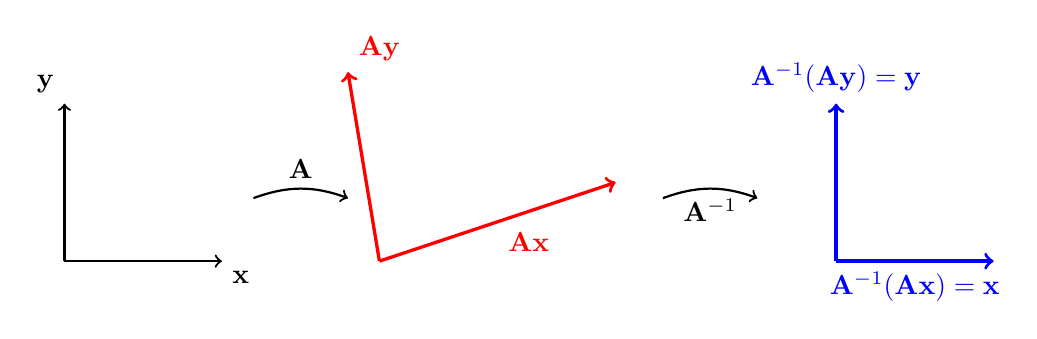
\begin{tikzpicture}[x=2cm,y=2cm]
 			
 			\begin{scope}
 				\draw[->, thick] (0,0) -- (1,0) node[below right] {${\bf x}$};
 				\draw[->, thick] (0,0) -- (0,1) node[above left] {${\bf y}$};
 			\end{scope}
 			
 			\begin{scope}[shift={(2.0,0)}]
 				\coordinate (A) at (1.5,0.5);
 				\coordinate (B) at (-0.2,1.2);
				\draw[->, very thick, red] (0,0) -- (A) node[pos=0.5, below right] {${\bf A}{\bf x}$};
 				\draw[->, very thick, red] (0,0) -- (B) node[above right] {${\bf A}{\bf y}$};
 			\end{scope}
 			
 			\begin{scope}[shift={(4.9,0)}]
 				\draw[->, very thick, blue] (0,0) -- (1,0) node[pos=0.5, below] {${\bf A}^{-1} ({\bf A}{\bf x}) = {\bf x}$};
 				\draw[->, very thick, blue] (0,0) -- (0,1) node[above] {${\bf A}^{-1} ({\bf A}{\bf y}) = {\bf y}$};
 			\end{scope}
 			
 			\draw[->, thick, bend left=20] (1.2,0.4) to node[above] {${\bf A}$} (1.8,0.4);
 			\draw[->, thick, bend left=20] (3.8,0.4) to node[below] {${\bf A}^{-1}$} (4.4,0.4);
 		\end{tikzpicture}
 		\caption{A matrix $\mathbf{A}$ represents a linear transformation of $\mathbb{R}^{2}$. The inverse matrix $\mathbf{A}^{-1}$ 
 			represents the inverse transformation. \label{fig_matrix_inverse_dict}} 
 		\end{figure}
		See also: matrix, determinant, linear regression, pseudoinverse.},
	first={inverse matrix},
		type=math,
	text={inverse matrix}
}

\newglossaryentry{matrix}
{name={matrix},
	description={A matrix\index{matrix} of size $m\times d$ is a 2-D array of numbers, 
 		which is denoted by 
		$$
  		{\bf A}= \begin{pmatrix}
   		A_{1,1} & A_{1,2} & \dots  & A_{1,d} \\
		A_{2,1} & A_{2,2} & \dots  & A_{2,d} \\
		\vdots  & \vdots  & \ddots & \vdots \\
		A_{m,1} & A_{m,2} & \dots  & A_{m,d}
		\end{pmatrix} \in \mathbb{R}^{m\times d}.
		$$
		Here, $A_{r,j}$ denotes the matrix entry in the $r$th row and the 
		$j$th column. Matrices are useful representations of various mathematical objects \cite{StrangLinAlg2016},
		including the following:
		\begin{itemize}
			\item Systems of linear equations: We can use a matrix to represent a system of linear equations 
			$$ \begin{pmatrix}
			A_{1,1} & A_{1,2} \\
			A_{2,1} & A_{2,2}
			\end{pmatrix}
			\begin{pmatrix}
				w_1 \\
				w_2
			\end{pmatrix}
			=\begin{pmatrix}
				y_1 \\
				y_2
			\end{pmatrix}
			\quad \text{ compactly as } \quad {\bf A}{\bf w}= {\bf y}.
			$$
    			One important example of systems of linear equations is the optimality condition for the 
    			model parameters within linear regression. 
			\item Linear maps:
			Consider a $d$-dimensional vector space $\mathcal{U}$ and a $m$-dimensional vector space $\mathcal{V}$. 
			If we fix a basis $\mathbf{u}^{(1)},\,\ldots,\,\mathbf{u}^{(d)}$ for $\mathcal{U}$ and a basis $\mathbf{v}^{(1)},\,\ldots,\,\mathbf{v}^{(m)}$ 
			for $\mathcal{V}$, each matrix ${\bf A}\in \mathbb{R}^{m\times d}$ naturally defines a 
			linear map $\alpha: \mathcal{U} \rightarrow \mathcal{V}$ (see Fig. \ref{fig_matrix_dict}) such that
   			$${\bf u}^{(j)} \mapsto \sum_{r=1}^{m} A_{r,j} {\bf v}^{(r)}.$$
			\item Datasets: We can use a matrix to represent a dataset. Each row 
			corresponds to a single data point, and each column corresponds to a specific 
			feature or label of a data point. 
		\end{itemize}
		\begin{figure}[H]
		\begin{center}
		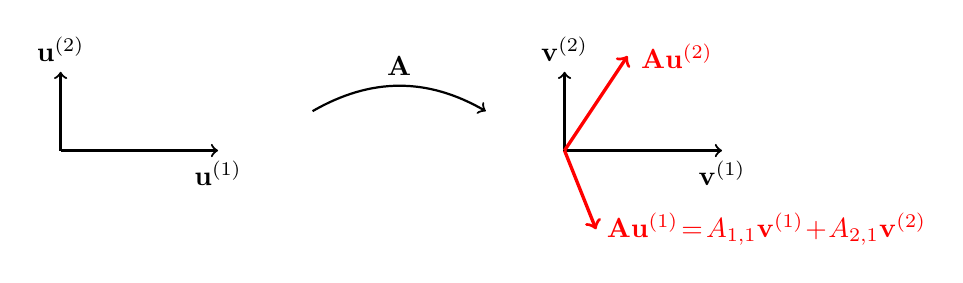
\begin{tikzpicture}[x=2cm]
			
			\begin{scope}
				\draw[->, thick] (0,0) -- (1,0) node[below] {${\bf u}^{(1)}$};
				\draw[->, thick] (0,0) -- (0,1) node[above] {${\bf u}^{(2)}$};
				
				
				
			\end{scope}
			
			\begin{scope}[shift={(3.2,0)}]
				\draw[->, thick] (0,0) -- (1,0) node[below] {${\bf v}^{(1)}$};
				\draw[->, thick] (0,0) -- (0,1) node[above] {${\bf v}^{(2)}$};
				\coordinate (A) at (0.2,-1.0);
				\coordinate (B) at (0.4,1.2);
				\draw[->, very thick, red] (0,0) -- (A) node[below,right] {${\bf A}{\bf u}^{(1)}\!=\!A_{1,1}{\bf v}^{(1)}\!+\!A_{2,1}{\bf v}^{(2)}$};
				\draw[->, very thick, red] (0,0) -- (B) node[right,xshift=1pt] {${\bf A}{\bf u}^{(2)}$};
				
				
			\end{scope}
			
			\draw[->, thick] (1.6,0.5) to[bend left] node[midway, above] {${\bf A}$} (2.7,0.5);
		
		\end{tikzpicture}
		\end{center}
		\caption{A matrix ${\bf A}$ defines a linear map between two vector spaces. \label{fig_matrix_dict}} 
		\end{figure}
		See also: linear map, dataset, linear model. },
	first={matrix},
	firstplural={matrices},
	type=math,
	plural={matrices},
	text={matrix}
}

\newglossaryentry{hyperplane}
{name={hyperplane},
	description={A hyperplane\index{hyperplane} is an $(d-1)$-dimensional affine 
				 subspace of a $d$-dimensional vector space. In the 
				 context of an Euclidean space $\mathbb{R}^{d}$, a 
				 hyperplane is a set of the form
 				 \[ \{ {\bf x}\in \mathbb{R}^d: {\bf w}^\top {\bf x}= b \},
  				 \]
                 where ${\bf w}\in \mathbb{R}^d \setminus \{0\}$ is a normal vector 
                 and $b \in \mathbb{R}$ is an offset. Such a hyperplane partitions 
				 $\mathbb{R}^d$ into two halfspaces
				\[\{ {\bf x}\in \mathbb{R}^d: {\bf w}^\top {\bf x}\leq b \} \quad 
				\text{and} \quad \{ {\bf x}\in \mathbb{R}^d: {\bf w}^\top {\bf x}\geq b \}.\]
 				Hyperplanes arise as the decision boundaries of linear classifiers.},
	first={hyperplane},
	type=math,
	plural={hyperplanes}, 
	firstplural={hyperplanes},
	text={hyperplane}
}

\newglossaryentry{normalvector}
{name={normal vector},
	description={See\index{normal vector} hyperplane.},
	first={normal vector},
	type=math,
	plural={normal vectors}, 
	firstplural={normal vectors},
	text={normal vector}
}

\newglossaryentry{halfspace}
{name={halfspace},
	description={See\index{halfspace} hyperplane.},
	first={halfspace},
	type=math,
	plural={halfspaces}, 
	firstplural={halfspaces},
	text={halfspace}
}



\newglossaryentry{subspace}
{name={subspace},
	description={A subset of a vector space $\mathcal{V}$ is a subspace\index{subspace} of $\mathcal{V}$ if it is also a 
		vector space with respect to the same operations as $\mathcal{V}$.
			   \\
		See also: vector space.},
	type=math, 
	first={subspace},
	text={subspace}
}

\newglossaryentry{columnspace}
{name={column space},
	description={The column space\index{column space} of a matrix 
		${\bf A}\in \mathbb{R}^{m\times d}$,
		denoted by ${\rm span}\left({\bf A}\right)$, is the set of all linear combinations of the 
		columns of ${\bf A}$. In other words, 
		$$ {\rm span}\left({\bf A}\right) = \{ {\bf A}{\bf w}: {\bf w}\in \mathbb{R}^{d} \}. $$
		The column space ${\rm span}\left({\bf A}\right)$ of the matrix ${\bf A}$ 
		is a subspace of the Euclidean space $\mathbb{R}^{m}$.
			   \\
		See also: matrix, vector space.},
	type=math,
	first={column space},
	text={column space}
}

\newglossaryentry{mvndist}
{name={multivariate normal distribution}, 
	description={The\index{multivariate normal distribution} multivariate normal distribution, 
		which is denoted by $\mathcal{N}\left({\bm \mu},{\bf C}\right)$, is a fundamental 
		probabilistic model for numerical feature vectors of fixed dimension $d$. 
		It defines a family of probability distributions over vector-valued random variables (RVs) 
		${\bf x}\in \mathbb{R}^{d}$~\cite{BertsekasProb}, \cite{GrayProbBook}, \cite{Lapidoth09}. 
		Each distribution in this family is fully specified by its mean vector 
		${\bm \mu}\in \mathbb{R}^{d}$ and covariance matrix 
		${\bf C}\in \mathbb{R}^{d\times d}$. When the 
		covariance matrix ${\bf C}$ is invertible, the corresponding probability distribution is 
		characterized by the following probability density function (pdf):
		\[p({\bf x}) = 
 		\frac{1}{\sqrt{(2\pi)^{d} \det\,({\bf C})}} 
 		\exp\left[ -\frac{1}{2} 
 		({\bf x}- {\bm \mu})\,^{T}\, {\bf C}^{-1} 
 		({\bf x}- {\bm \mu}) \right].
 		\]
		Note that this probability density function (pdf) is only defined when ${\bf C}$ is invertible.
   		More generally, any random variable (RV) ${\bf x}\sim \mathcal{N}\left({\bm \mu},{\bf C}\right)$ 
   		admits the following representation:
  		\[
    		{\bf x}= {\bf A}{\bf z}+ {\bm \mu}\]
   		where ${\bf z}\sim \mathcal{N}\left(\mathbf{0},\mathbf{I}\right)$ is a standard normal random vector 
   		and ${\bf A}\in \mathbb{R}^{d\times d}$ satisfies ${\bf A}{\bf A}^\top = {\bf C}$. 
   		This representation remains valid even when ${\bf C}$ is singular, in which case ${\bf A}$ 
   		is not full rank~\cite[Ch. 23]{Lapidoth2017}.
   		The family of multivariate normal distributions is exceptional among probabilistic models for numerical 
   		quantities, at least for the following reasons. First, the family is closed under affine 
   		transformations, i.e.,
		\[ 
		{\bf x}\sim \mathcal{N}({\bm \mu},{\bf C}) \mbox{ implies } 
		{\bf B}{\bf x}\!+\!{\bf c}\sim \mathcal{N}\big( {\bf B}{\bm \mu}+{\bf c},{\bf B}{\bf C}{\bf B}\,^{T} \big). 
		\]
		Second, the probability distribution $\mathcal{N}(\mathbf{0},{\bf C})$ maximizes the 
		differential entropy among all distributions with the same covariance matrix ${\bf C}$~\cite{coverthomas}. 
		\\ 
		See also: probabilistic model, probability distribution, standard normal random vector, differential entropy, Gaussian random variable (Gaussian RV).}, 
	first={multivariate normal distribution},
	type=math, 
	text={multivariate normal distribution}
}

\newglossaryentry{stdnormvec}
{name={standard normal random vector}, 
	description={A\index{standard normal vector} standard normal random vector is a random 
		vector ${\bf x}=\big(x_{1}, \,\ldots, \,x_{d}\big)\,^{T}$ 
		whose entries are independent and identically distributed (i.i.d.) Gaussian random variables (Gaussian RVs) $x_{j} \sim \mathcal{N}(0,1)$. 
		It is a special case of a multivariate normal distribution, ${\bf x}\sim \mathcal(\mathbf{0},\mathbf{I})$.
		\\ 
		See also: vector, independent and identically distributed (i.i.d.), Gaussian random variable (Gaussian RV), multivariate normal distribution, random variable (RV).}, 
	first={standard normal random vector},
	type=math, 
	text={standard normal random vector}
}

\newglossaryentry{continuous}
{name={continuous}, 
	description={A function\index{continuous} $f: \mathbb{R}^{d} \to \mathbb{R}$ is 
		continuous at a point ${\bf x}' \in \mathbb{R}^{d}$ if, for 
	 	every $\epsilon > 0$, there is a $\delta > 0$ such that, for all 
	 	${\bf x}\in \mathbb{R}^{d}$ with $\mleft\lVert {\bf x}- {\bf x}' \mright\rVert_{2} < \delta$, 
	 	it holds that $|f({\bf x}) - f({\bf x}')| < \epsilon$ \cite{RudinBookPrinciplesMatheAnalysis}. 
	 	In other words, we can make $f({\bf x})$ arbitrarily close to $f({\bf x}')$ 
	 	by choosing ${\bf x}$ sufficiently close to ${\bf x}'$. 
		\begin{figure}[htbp]
		\centering
	 	\begin{tikzpicture}[
		>=stealth, 
    	thick,
		
    	declare function={f(\x) = 0.3*(\x-2)^3 + 2.5;}
			]
		\def\xprime{2}      
    	\def\epsilonval{1.2}   
		\def\deltaval{1.3}     
		\def\xmax{5.5}
		\def\ymax{5}
		\fill[blue!5] (0, {f(\xprime)-\epsilonval}) rectangle (\xmax, {f(\xprime)+\epsilonval});
		\draw[blue!30, dashed] (0, {f(\xprime)-\epsilonval}) -- (\xmax, {f(\xprime)-\epsilonval});
		\draw[blue!30, dashed] (0, {f(\xprime)+\epsilonval}) -- (\xmax, {f(\xprime)+\epsilonval});
		\fill[red!10] ({\xprime-\deltaval}, 0) rectangle ({\xprime+\deltaval}, \ymax);
		\draw[red!40, dashed] ({\xprime-\deltaval}, 0) -- ({\xprime-\deltaval}, \ymax);
		\draw[red!40, dashed] ({\xprime+\deltaval}, 0) -- ({\xprime+\deltaval}, \ymax);
		\fill[purple!20] ({\xprime-\deltaval}, {f(\xprime)-\epsilonval}) rectangle ({\xprime+\deltaval}, {f(\xprime)+\epsilonval});
		\draw[purple, thick] ({\xprime-\deltaval}, {f(\xprime)-\epsilonval}) rectangle ({\xprime+\deltaval}, {f(\xprime)+\epsilonval});
		\draw[->] (-0.5,0) -- (\xmax,0) node[right] {$x$};
		\draw[->] (0,-0.5) -- (0,\ymax) node[above] {};
		
		\draw[line width=1.5pt, black!80] plot[domain=0.2:4.5, samples=100] (\x, {f(\x)}) 
			node[right] {$f(x)$};
		\draw[dashed] (\xprime, 0) -- (\xprime, {f(\xprime)}) -- (0, {f(\xprime)});
		\fill[black] (\xprime, {f(\xprime)}) circle (2pt);
		\node[below,yshift=-5pt] at (\xprime, 0) {$x'$};
		\node[left] at (0, {f(\xprime)}) {$f(x')$};
		\draw[decorate, decoration={brace, amplitude=4pt}, blue!80] 
		(-0.2, {f(\xprime)}) -- (-0.2, {f(\xprime)+\epsilonval}) 
		node[midway, left=4pt] {$\varepsilon$};
		\draw[decorate, decoration={brace, amplitude=4pt}, blue!80] 
		(-0.2, {f(\xprime)-\epsilonval}) -- (-0.2, {f(\xprime)}) 
		node[midway, left=4pt] {$\varepsilon$};
		\draw[decorate, decoration={brace, amplitude=4pt, mirror}, red!80] 
		(\xprime, -0.2) -- ({\xprime+\deltaval}, -0.2) 
		node[midway, below=4pt] {$\delta$};
		\draw[decorate, decoration={brace, amplitude=4pt, mirror}, red!80] 
		({\xprime-\deltaval}, -0.2) -- (\xprime, -0.2) 
		node[midway, below=4pt] {$\delta$};
		\node[align=left, purple!40!black, font=\small] at (6.2, 1.5) 
		{If $| x- x' | < \delta$\\
		then $| f(x) - f(x') | < \varepsilon$};
		\end{tikzpicture}
		\caption{The function $f(x) = 0.3(x-2)^3 + 2.5$ is continuous 
		         at every $x'$.}
		\end{figure}
		If $f$ is continuous 
	 	at every point ${\bf x}' \in \mathbb{R}^{d}$, then $f$ is said to be 
	 	continuous on $\mathbb{R}^{d}$. The notion of a continuous 
	 	function can be naturally extended to functions between general metric spaces 
		\cite{RudinBookPrinciplesMatheAnalysis}.
		\\
		See also: Euclidean space, metric.},
	first={continuous},
	type=math,
	text={continuous}
}

\newglossaryentry{minimum}
{name={minimum},
	description={Given a set of real numbers, the minimum\index{minimum} is the smallest of those numbers.
		Note that for some sets, such as the set of negative real numbers, the minimum does not exist.},
	firstplural={minima}, 
 	plural={minima},
	type=math, 
	first={minimum},
	text={minimum}
}

\newglossaryentry{co-domain}
{name={co-domain}, 
	description={The co-domain\index{co-domain} of a function 
		$f: \mathcal{U} \rightarrow \mathcal{V}$ is the set $\mathcal{V}$ 
		into which $f$ maps elements of its domain $\mathcal{U}$.  
		\begin{figure}[H]
			\centering
		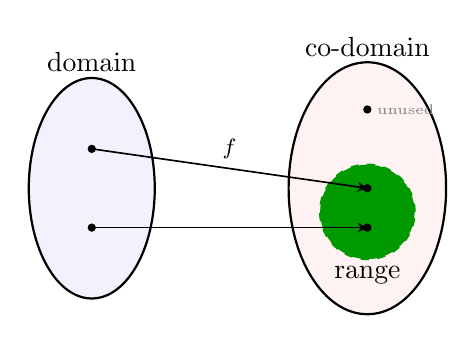
\begin{tikzpicture}[
			>=stealth, 
			node distance=2cm,
			scale=1.0, every node/.style={transform shape} 
		]
			
			\draw[thick, fill=blue!5] (0,0) ellipse (0.8cm and 1.4cm);
			\node[] at (0, 1.6) {domain};
			
			\draw[thick, fill=red!5] (3.5,0) ellipse (1cm and 1.6cm);
			\node[] at (3.5, 1.8) {co-domain};
			\draw[dashed, fill=green!10, thick, green!60!black] (3.5, -0.3) circle (0.6cm);
			\node[] at (3.5, -1.1) {range};
			\fill (0, 0.5) circle (1.5pt) coordinate (a1);
			\fill (0, -0.5) circle (1.5pt) coordinate (a2);
			
			\fill (3.5, 0) circle (1.5pt) coordinate (b1);
			\fill (3.5, -0.5) circle (1.5pt) coordinate (b2);
			
			\fill (3.5, 1.0) circle (1.5pt) coordinate (b_miss) node[right, font=\tiny, gray] {unused};
			\draw[->, semithick] (a1) -- (b1);
			\draw[->, semithick] (a2) -- (b2);
			
			\node[font=\footnotesize] at (1.75, 0.5) {$f$};
		\end{tikzpicture}
	\end{figure}
		See also: domain, function, map.},
	first={co-domain},
	firstplural={co-domains}, 
	type=math, 
	plural={co-domains},
	text={co-domain}
}


\newglossaryentry{cdf}
{name={cumulative distribution function (cdf)},
	description={The \index{cumulative distribution function (cdf)} cdf 
		$F^{(x)}\left(\eta\right)$ of a real-valued random variable (RV) $x$ is \cite{AshProbMeasure}, \cite{papoulis}
		$$F^{(x)}\left(\eta\right) :=\mathbb{P}\left(x\leq \eta\right).$$
					\\ 
		See also: random variable (RV), probability density function (pdf), probability distribution.},
	first={cumulative distribution function (cdf)},
	firstplural={cumulative distribution functions (cdfs)}, 
	plural={cdfs}, 
	type=math,
	text={cdf} 
}

\newglossaryentry{weightedgraph}
{name={weighted graph},
	description={A graph\index{weighted graph} whose edges 
	are assigned numeric weights. Typically, these edge weights 
	are nonnegative real numbers. For example, if a graph represents 
	a road network with nodes being intersections and edges representing 
	road segments, the edge weight could represent the capacity (measured 
	in maximum vehicles per hour) of the road segment \cite{NewmannBook}.  
	\begin{figure}[htbp] 
				\centering
			  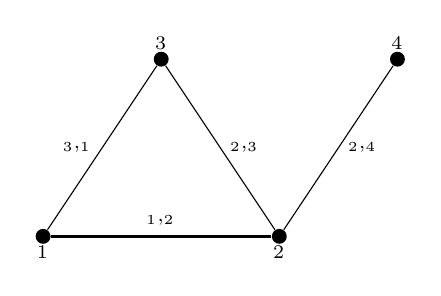
\begin{tikzpicture}[scale=1.5,
					node/.style={circle, fill=black, inner sep=1.9pt},
					lab/.style={anchor=west, xshift=3pt}
					]
					
					\node[node] (v1) at (0,0) {};
					\node[node] (v2) at (2,0) {};
					\node[node] (v3) at (1,1.5) {};
					\node[node] (v4) at (3,1.5) {};
					
					\node[anchor=north] at (v1) {$\nodeidx_1$};
					\node[anchor=north] at (v2) {$\nodeidx_2$};
					\node[anchor=south] at (v3) {$\nodeidx_3$};
					\node[anchor=south] at (v4) {$\nodeidx_4$};
					
					\draw [line width=1pt] (v1) -- node[midway, above] {$\edgeweight_{\nodeidx_1,\nodeidx_2}$} (v2);
					\draw (v2) -- node[midway, right] {$\edgeweight_{\nodeidx_2,\nodeidx_3}$} (v3);
					\draw (v3) -- node[midway, left] {$\edgeweight_{\nodeidx_3,\nodeidx_1}$} (v1);
					\draw (v2) -- node[midway, right] {$\edgeweight_{\nodeidx_2,\nodeidx_4}$} (v4);
				\end{tikzpicture}
				\caption{A weighted graph with four nodes 
				$\mathcal{V}= \{\nodeidx_1, \nodeidx_2, \nodeidx_3, \nodeidx_4\}$ 
				and four edges $\mathcal{E}= \{\{\nodeidx_1,\nodeidx_2\},
				\{\nodeidx_2,\nodeidx_3\}, \{\nodeidx_3,\nodeidx_1\}, 
				\{\nodeidx_2,\nodeidx_4\}\}$. Each edge is assigned a weight.}
			\end{figure}		
		See also: graph.},
	first={weighted graph},
	type=math,
	firstplural={weighted graphs}, 
	plural={weighted graphs}, 
	text={weighted graph} 
}

\newglossaryentry{graph}
{name={graph},
 description={A graph\index{graph} $\mathcal{G}= \left( \mathcal{V},\mathcal{E}\right)$ 
              consists of a node set $\mathcal{V}$ and an edge set $\mathcal{E}$.
			  Each edge $e\in \mathcal{E}$ is characterized by the nodes to which 
			  it is connected and in what precise sense. For example, 
			  an edge of a directed graph is leaving one node 
			  and pointing to another node. An edge of an undirected 
			  graph connects two nodes without any sense of 
			  direction \cite{NewmannBook,RockNetworks}. 
			  In principle, there can also be several (parallel) edges that are 
			  connected to the same nodes in the same way \cite{RockNetworks}. 
			  Moreover, edges may connect a node to itself, resulting in 
			  so-called self-loops \cite{NewmannBook}. 
			  A simple undirected graph contains no 
			  parallel edges and no self-loops \cite{WilsonGraph2010}. 
			  Each edge $e\in \mathcal{E}$ of a simple undirected 
			  graph can be identified with a set of two nodes ${i,i'}$. 
			  \begin{figure}[htbp] 
				\centering
			  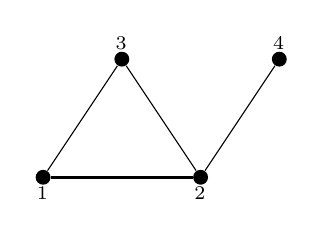
\begin{tikzpicture}[scale=1,
					node/.style={circle, fill=black, inner sep=1.9pt},
					lab/.style={anchor=west, xshift=3pt}
					]
					
					\node[node] (v1) at (0,0) {};
					\node[node] (v2) at (2,0) {};
					\node[node] (v3) at (1,1.5) {};
					\node[node] (v4) at (3,1.5) {};
					
					\node[anchor=north] at (v1) {$\nodeidx_1$};
					\node[anchor=north] at (v2) {$\nodeidx_2$};
					\node[anchor=south] at (v3) {$\nodeidx_3$};
					\node[anchor=south] at (v4) {$\nodeidx_4$};
					
					\draw [line width=1pt] (v1) -- (v2);
					\draw (v2) -- (v3);
					\draw (v3) -- (v1);
					\draw (v2) -- (v4);
				\end{tikzpicture}
				\caption{A simple undirected graph with four nodes 
				$\mathcal{V}= \{\nodeidx_1, \nodeidx_2, \nodeidx_3, \nodeidx_4\}$ 
				and four edges $\mathcal{E}= \{\{\nodeidx_1,\nodeidx_2\},
				\{\nodeidx_2,\nodeidx_3\}, \{\nodeidx_3,\nodeidx_1\}, 
				\{\nodeidx_2,\nodeidx_4\}\}$.}
			\end{figure}
		      Weighted graphs assign a numerical value $\edgeweight_{e}$, 
			  referred to as edge weight, to each edge $e\in \mathcal{E}$.
					\\ 
		See also: map, weights.},
 first={graph},
 text={graph}, 
 firstplural={graphs}, 
 plural={graphs}, 
 type=math
}

\newglossaryentry{markovchain}
{name={Markov chain},
  description={A Markov chain\index{Markov chain} is a stochastic process $\{X_t\}_{t\in \mathbb{N}}$, 
               defined on a common probability space and using the index set $\mathbb{N}$. The 
			   random variable (RV) $X_t$ might represent (the generation of) a state of a physical system 
			   at the time instant $t$. The defining property of a Markov chain 
			   is the Markov property \cite{NorrisMarkovChains1997,durrett2010probability,papoulis}: 
			   For all $t\in \mathbb{N}$,
 			   \begin{equation}
 				\nonumber \mathbb{P}^{(X_{t+1} \mid X_t,\ldots,X_1)} = \mathbb{P}^{(X_{t+1} \mid X_t)}. 
 				\end{equation}
 			    In other words, the conditional probability distribution of the next state $X_{t+1}$ 
				depends on the past $X_{t},X_{t-1},\dots,X_{1}$ 
				only through the current state $X_{t}$. The concept of a 
				Markov chain can be generalized from discrete time (with index set $\mathbb{N}$) 
				to continuous time (with index set $\mathbb{R}$) \cite{NorrisMarkovChains1997}. \\ 
				See also: stochastic process, conditional probability distribution.},
    first={Markov chain},
    type=math,
    text={Markov chain}, 
	plural={Markov chains}, 
	firstplural={Markov chains}
}

\newglossaryentry{markovprop}
{name={Markov property},
  description={See Markov chain\index{Markov property}.},
    first={Markov property},
    type=math,
    text={Markov property}
}

\newglossaryentry{em}
{name={expectation–maximization (EM)}, 
	description={\index{expectation–maximization (EM)}
	    The EM algorithm \cite{dempster1977maximum} is an iterative optimization method for 
		approximately solving certain maximum likelihood optimization problems 
		that are difficult to solve directly \cite[Sec. 9.4]{BishopBook}, \cite[Sec. 11.4.7]{Murphy2012}.
	    To motivate the EM algorithm and explain its construction, 
		consider a machine learning (ML) application involving a single observed data point 
		with feature $x\in \mathcal{X}$, where $\mathcal{X}$ 
		is a finite feature space. The data generation 
		is modeled via a probabilistic model that consists of a random variable (RV) $x'$ 
		with probability mass function (pmf) $p^{(x')}\left(\cdot;{\bf w}\right)$. Here, 
		the actual model parameters ${\bf w}\in \mathcal{W}$ - used for the data 
		generation via sampling from $p^{(x')}\left(\cdot;{\bf w}\right)$ - are unknown. A widely 
		used approach for estimating these model parameters is via the solutions of the maximum likelihood 
		problem
		\begin{equation}
			\label{equ_def_ML_EM_dict}
			\min_{{\bf w}\in \mathcal{W}} - \log p^{(x')}\left(x;{\bf w}\right).
		\end{equation}
		For some probabilistic models, such as a Gaussian mixture model (GMM), this optimization problem can be 
		difficult to solve directly. As a work-around, one can often introduce an auxiliary 
		attribute $y\in \mathcal{Y}$, generated via some random variable (RV) $y'$, 
		such that the corresponding probabilistic model $p^{(x',y')}\left(\cdot,\cdot;{\bf w}\right)$ 
		yields a much easier maximum likelihood problem 
		\begin{equation}
			\label{equ_def_complete_EM_dict}
			\min_{{\bf w}\in \mathcal{W}} 
			- \log p^{(x',y')}\left(x,y;{\bf w}\right).
		\end{equation}
		The attribute $y$ is introduced solely to simplify 
		\eqref{equ_def_complete_EM_dict}, but it is not observed in practice—only the 
		feature $x$ is available. Thus, we cannot solve \eqref{equ_def_complete_EM_dict} 
		directly as we do not know which value $y$ to plug into the probability mass function (pmf) 
		$ p^{(x',y')}\left(x,y;{\bf w}\right)$. 
		The EM method resolves this dilemma by alternating between two steps:
		\begin{itemize}
			\item {\bf (E-step)} computing a “soft’’ estimate of the auxiliary 
			attribute $y$ in the form of the posterior 
			$p^{(y'|x')}\left(\cdot;\widehat{{\bf w}}\right)$
			using the current choice $\widehat{{\bf w}}$ for the model parameters, and 
			\item {\bf (M-step)} minimizing a surrogate objective function derived from this posterior.
		\end{itemize}
		The completion of these two steps constitutes one full iteration of 
		the EM method. 
		In more detail, the E-step produces the function
		\[
		Q({\bf w}\mid \widehat{{\bf w}})
		:=- \sum_{y\in \mathcal{Y}} 
		p^{(y'|x')}\left(y;\widehat{{\bf w}}\right)
		\log\!\Big(
		p^{(x',y')}\left(x,y;{\bf w}\right)
		/p^{(y'|x')}\left(y;\widehat{{\bf w}}\right)
		\Big),
		\]
		and the M-step minimizes $Q({\bf w}\mid \widehat{{\bf w}})$ over 
		${\bf w}\in \mathcal{W}$.
		This function satisfies two key properties \cite[Sec. 9.4]{BishopBook},\cite[Sec. 11.4.7]{Murphy2012}:
		\begin{itemize}
			\item {\bf Upper bound:}
			\begin{equation}
				\label{equ_upper_bound_EM_dict}
				Q({\bf w}\mid \widehat{{\bf w}})
				\geq
				- \log p^{(x')}\left(x;{\bf w}\right)
				\quad \text{for all } {\bf w}\in \mathcal{W}.
			\end{equation}
			\item {\bf Tightness:}
			\begin{equation}
				\label{equ_upper_bound_EM_dict_tight}
				Q(\widehat{{\bf w}}\mid \widehat{{\bf w}})
				=- \log p^{(x')}\left(x;\widehat{{\bf w}}\right).
			\end{equation}
		\end{itemize}
		To summarize, during each iteration, EM minimizes an upper-bounding 
		surrogate objective function that is tight at the current iterate $\widehat{{\bf w}}$. 
		Thus, EM is a majorize–minimize (MM) method for approximately solving \eqref{equ_def_ML_EM_dict}. 
		The above construction and analysis of EM can be extended to more 
		general settings involving multiple data points 
		and infinite feature spaces such as $\mathbb{R}^{d}$; see \cite[Sec. 11.4.7]{Murphy2012} for details. 
			\\
		See also: probabilistic model, maximum likelihood, optimization problem. },
	first={expectation-maximization (EM)},
	type=math, 
	text={EM}
}

\newglossaryentry{ppca}
{name={probabilistic principal component analysis (PPCA)}, 
	description={PPCA\index{probabilistic principal component analysis (PPCA)} 
		extends\linebreak basic principal component analysis (PCA) by using a probabilistic model for data points. 
		The probabilistic model of PPCA frames the task of dimensionality reduction 
		as an estimation problem that can be solved using expectation-maximization (EM) \cite{TippingProbPCA}.
				\\
		See also: principal component analysis (PCA), probabilistic model, dimensionality reduction, expectation-maximization (EM).},
	first={probabilistic principal component analysis (PPCA)},
	type=math, 
	text={PPCA}
}

\newglossaryentry{condprobdist}
{name={conditional probability distribution}, 
	description={Consider\index{conditional probability distribution} 
     		a stochastic process consisting of two random variables (RVs) ${\bf x}$ and $y$ 
    		with probability distribution $\mathbb{P}^{({\bf x},y)}$. The conditional 
    		probability distribution of $y$ given (or conditioned on) ${\bf x}$ is 
    		denoted by $\mathbb{P}^{(y\mid{\bf x})}$. It is defined via the 
    		conditional expectations of the indicator functions of  
    		measurable sets in the $\sigma$-algebra generated by 
    		the random variable (RV) $y$ \cite{BillingsleyProbMeasure}, \cite{KallenbergBook}.
		\\
		See also: probability distribution, conditional expectation. },
  	first={conditional probability distribution}, 
  	plural={conditional probability distributions},
  	type=math, 
  	text={conditional probability distribution}
}

\newglossaryentry{linearmap}
{name={linear map}, plural={linear maps}, 
	description={A\index{linear map} linear map 
	             $f: \mathbb{R}^d\rightarrow \mathbb{R}^m$ 
	    is a function that satisfies additivity, i.e.,
		$f({\bf x}+ {\bf y}) = f({\bf x}) + f({\bf y})$, and homogeneity, i.e.,
		$f(c{\bf x}) = c f({\bf x})$, for all vectors ${\bf x}, {\bf y}\in \mathbb{R}^d$ 
		and scalars $c \in \mathbb{R}$. In particular, $f(\mathbf{0}) = \mathbf{0}$. 
		Any linear map can be represented as a matrix multiplication 
		$f({\bf x}) = {\bf A}{\bf x}$ for some matrix ${\bf A}\in \mathbb{R}^{m \times n}$. 
		The collection of real-valued linear maps (where $m=1$) 
		for a given dimension $d$ constitute a linear model. The notion 
		of a linear map can be generalized from domain $\mathbb{R}^{d}$ 
		and co-domain $\mathbb{R}^{m}$ to arbirary vector spaces.
		\\
		See also: map, function, vector, matrix, linear model.},
	first={linear map},
	type=math, 
	plural={linear maps}, 
	firstplural={linear maps}, 
	text={linear map}
}

\newglossaryentry{vector}
{name={vector},
	description={A\index{vector} vector is an element of a vector space. 
		In the context of machine learning (ML), a particularly important example of a vector space 
		is the Euclidean space $\mathbb{R}^{d}$, where $d\in \mathbb{N}$ 
		is the (finite) dimension of the space. A vector ${\bf x}\in \mathbb{R}^{d}$ 
		can be represented as a list or one-dimensional (1-D) array of real numbers, i.e., 
		$x_1, \,\ldots, \,x_{d}$ with $x_j\in \mathbb{R}$ for 
		$j= 1, \,\ldots, \,d$. The value $x_j$ is the $j$th 
		entry of the vector ${\bf x}$. It can also be useful to view a vector ${\bf x}\in \mathbb{R}^{d}$ 
		as a function that maps each index $j\in \{1, \,\ldots, \,d\}$ 
		to a value $x_j\in \mathbb{R}$, i.e., ${\bf x}: j\mapsto x_j$. 
		This perspective is particularly useful for the study of kernel methods. See Fig. 
		\ref{fig:vector-function-dual_dict} for the two views of a vector.
		\begin{figure}[H]
			
			\begin{minipage}[c]{0.48\textwidth}
				\centering 
				2, --1, 3, 0, --2, 1
				\begin{minipage}{\textwidth}
				\vspace{5ex}
				\centering
				{\selectfont (a)}
				\end{minipage}
			\end{minipage}
			\hfill
			
			\begin{minipage}{0.48\textwidth}
			\centering
			\begin{tikzpicture}
			\begin{axis}[
    				width=6.5cm,
    				height=5cm,
    				title={},
    				xlabel={index $j$},
    				ylabel={$x_j$},
   		 		ymin=-3.5, ymax=3.5,
    				xmin=0.5, xmax=6.5,
   	 			xtick={1,2,3,4,5,6},
    				ytick={-3,-2,-1,0,1,2,3},
    				axis x line=bottom,        
    				axis y line=left,          
    				grid=both,
    				major grid style={dotted, gray!60},
    				enlargelimits=0.1
			]
			\addplot+[ycomb, thick, mark=*]
    			coordinates {
        				(1,2)
        				(2,-1)
       	 			(3,3)
        				(4,0)
        				(5,-2)
        				(6,1)
    			};
			\end{axis}
			\node at (2,-2.5) {(b)};
			\end{tikzpicture}
			\end{minipage}
			\caption{Two equivalent views of a vector ${\bf x}= \big( 2, -1, 3, 0, -2, 1 \big)^{T} \in \mathbb{R}^{6}$.
			(a) As a numeric array. (b) As a map $j\mapsto x_j$.}
			\label{fig:vector-function-dual_dict}
		\end{figure}
		See also: vector space, Euclidean space, linear map.},
	first={vector},
	firstplural={vectors},
	type=math,
	plural={vectors},
	text={vector}
}

\newglossaryentry{vectorspace}
{name={vector space},
	description={A\index{vector space} vector space $\mathcal{V}$ (also called linear space) 
		is a collection of elements, called vectors, along with the following two operations 
		(see also Fig. \ref{fig:vector-ops_dict}): 
    		1) addition (denoted by ${\bf v}+{\bf w}$) of two vectors ${\bf v},{\bf w}$; and 2) multiplication 
		(denoted by $c \,\cdot \,{\bf v}$) of a vector ${\bf v}$ with a scalar $c$ that belongs to some 
		number field (such as the real numbers $\mathbb{R}$ or the complex numbers $\mathbb{C}$). The defining 
		property of a vector space is that it is closed under two specific operations. First, 
		if ${\bf v}, {\bf w}\in \mathcal{V}$, then ${\bf v}+ {\bf w}\in \mathcal{V}$. Second, if ${\bf v}\in \mathcal{V}$ 
		and $c \in \mathbb{R}$, then $c {\bf v}\in \mathcal{V}$.
		\begin{figure}[H]
		\centering
			\begin{tikzpicture}[>=Stealth, scale=1.2]
			
  			\coordinate (O) at (0,0);            
  			\coordinate (V) at (2,1.5);          
  			\coordinate (W) at (1,3);            
  			\coordinate (VplusW) at (3,4.5);     
  			\coordinate (HalfV) at (1,0.75);     
  			\draw[->, thick, blue] (O) -- (V) node[pos=1, right] {${\bf v}$};
  			\draw[->, thick, red] (O) -- (W) node[pos=1, left] {${\bf w}$};
  			\draw[->, thick, purple] (O) -- (VplusW) node[pos=0.99, above right] {${\bf v}+{\bf w}$};
  			\draw[dashed, red] (V) -- (VplusW);
  			\draw[dashed, blue] (W) -- (VplusW);
  			\draw[->, thick, orange] (O) -- (HalfV) node[midway, right] {$ \alpha {\bf v}$};
			
  			\filldraw[black] (O) circle (2pt) node[below left] {$\mathbf{0}$};  
  			\filldraw[blue] (V) circle (2pt);         
  			\filldraw[red] (W) circle (2pt);          
  			\filldraw[purple] (VplusW) circle (2pt);  
  			\filldraw[orange] (HalfV) circle (2pt);   
			\end{tikzpicture}
			\caption{A vector space $\mathcal{V}$ is a collection of vectors such that 
			scaling and adding them always yields another vector in $\mathcal{V}$.}
			
			
			\label{fig:vector-ops_dict}
		\end{figure}
		A common example of a vector space is the Euclidean space $\mathbb{R}^n$, which is 
		widely used in machine learning (ML) to represent datasets. We can also use $\mathbb{R}^n$ 
		to represent, either exactly or approximately, the hypothesis space used by an machine learning (ML) method.  
		Another example of a vector space, which is naturally associated with every probability space 
		$\big(\Omega,\mathcal{F},\mathbb{P}\left(\cdot\right) \big)$, is the collection of all 
		real-valued random variables (RVs) $x: \Omega\rightarrow \mathbb{R}$ \cite{RudinBook}, \cite{folland1999real}.  
		\\
		See also: vector, Euclidean space, linear model, linear map.},
	first={vector space},
	plural={vector spaces}, 
	firstplural={vector spaces}, 
	type=math,
	text={vector space}
}


\newglossaryentry{stochastic}
{name={stochastic},
	description={We refer to a\index{stochastic} method as stochastic if it involves a 
		random component or is governed by probabilistic laws. Machine learning (ML) methods use randomness 
		to reduce computational complexity (e.g., see stochastic gradient descent (SGD)) or 
		to capture uncertainty in probabilistic models.
		\\
		See also: stochastic gradient descent (SGD), uncertainty, probabilistic model.},
	first={stochastic},
	type=math, 
	text={stochastic}
}

\newglossaryentry{stochproc}
{name={stochastic process},
	description={A stochastic process\index{stochastic process} is a collection of 
		random variables (RVs) defined on a common probability space and indexed by some set 
		$\mathcal{I}$ \cite{GrayProbBook}, \cite{papoulis}, \cite{Brockwell91}. The index set 
		$\mathcal{I}$ typically represents time or space, allowing us to represent 
		random phenomena that evolve across time or spatial dimensions—for example, 
		sensor noise or financial time series. Stochastic processes are not limited 
		to temporal or spatial settings. For instance, random graphs such as 
		the Erd\H{o}s–R\'enyi graph (ER graph) or the stochastic block model (SBM) can also be viewed as stochastic processes. 
		Here, the index set $\mathcal{I}$ consists of node pairs that index random variables (RVs) whose values 
		encode the presence or weight of an edge between two nodes. Moreover, stochastic 
		processes naturally arise in the analysis of stochastic algorithms, 
		such as stochastic gradient descent (SGD), which construct a sequence of random variables (RVs). 
		\\
		See also:  random variable (RV), stochastic block model (SBM), stochastic gradient descent (SGD), uncertainty, probabilistic model.},
	first={stochastic process},
	firstplural={stochastic processes},
	type=math, 
	plural={stochastic processes},
	text={stochastic process}
}

\newglossaryentry{characteristicfunc}
{name={characteristic function},
	description={The characteristic function\index{characteristic function} 
		of a real-valued random variable (RV) $x$ is the function \cite[Sec. 26]{BillingsleyProbMeasure}
		$$ \phi_{x}(t) :=\mathbb{E} { \exp\,(j t x) } \mbox{ with } j = \sqrt{-1}.$$
	 	The characteristic function uniquely determines the probability distribution of $x$. 
		\\
		See also: random variable (RV), probability distribution.},
	first={characteristic function},
	firstplural={characteristic functions}, 
	type=math, 
	plural={characteristic functions},
	text={characteristic function}
}

\newglossaryentry{entropy}
{name={entropy},
	description={Entropy\index{entropy} quantifies the uncertainty or 
		unpredictability associated with an random variable (RV) \cite{coverthomas}. 
		For a discrete random variable (discrete RV) $x$ taking on values in a finite set 
		$\mathcal{S} = \{x_1, \,\ldots, \,x_k\}$ with 
		a probability mass function (pmf) $p^{(x)}\left(x_{c}\right) (=\mathbb{P}\left(x = x_{c}\right))$, 
		the entropy is defined as \cite{coverthomas}
		\[
		   H\left(x\right) :=-\sum_{c=1}^{k} p^{(x)}\left(x_{c}\right)  \log p^{(x)}\left(x_{c}\right) .
		\]
		For a given set of values $\mathcal{S}$, the entropy is maximized for a 
		uniformly distributed random variable (RV), where $p^{(x)}\left(x_{c}\right)=1/k$. 
		The minimal entropy, which is zero, is obtained when $p^{(x)}\left(x_{c}\right)=1$ 
		for some $x_{c} \in \mathcal{S}$.
		Differential entropy generalizes the concept of entropy from discrete random variables (discrete RVs) to 
		continuous random variables (RVs). 
		\\
		See also: uncertainty, probabilistic model.},
	first={entropy},
	type=math, 
	text={entropy}
}

\newglossaryentry{diffentropy}
{name={differential entropy},
	description={For\index{differential entropy} a 
	random variable (RV) ${\bf x}\in \mathbb{R}^{d}$ 
	with a probability density function (pdf) $p^{(x)}\left(\cdot\right)$, the differential entropy 
	is defined as \cite{coverthomas}
		\[
		h({\bf x}) :=- \int_{{\bf x}' \in \mathbb{R}^{d}} \log p({\bf x}') \, d p^{({\bf x})}\left({\bf x}'\right) .
		\]
	Differential entropy can be negative and lacks some properties of 
	entropy for discrete-valued random variables (RVs), such as invariance under 
	a change of variables \cite{coverthomas}. Among all random variables (RVs) with a 
	given mean ${\bm \mu}$ and covariance matrix ${\bf C}$, 
	$h({\bf x})$ is maximized by ${\bf x}\sim \mathcal{N}\left({\bm \mu},{\bf C}\right)$. 
		\\
		See also: uncertainty, probabilistic model.},
	first={differential entropy},
	type=math,
	text={differential entropy}
}


\newglossaryentry{domain}
{name={domain}, 
	description={The domain\index{domain} of a function 
		$f: \mathcal{U} \rightarrow \mathcal{V}$ is the set $\mathcal{U}$ 
		from which $f$ takes its inputs.  
		\\
		See also: function, co-domain, map.},
	first={domain},
	firstplural={domains}, 
	type=math, 
	plural={domains},
	text={domain}
}

\newglossaryentry{function}
{name={function}, 
	description={A function\index{function} between two sets $\mathcal{U}$ and $\mathcal{V}$ assigns  
		each element $u \in \mathcal{U}$ exactly one element $f(u) \in \mathcal{V}$ \cite{RudinBookPrinciplesMatheAnalysis}.
		We write this as $$f: \mathcal{U} \rightarrow \mathcal{V}: u \mapsto f(u)$$ 
		where $\mathcal{U}$ is the domain and $\mathcal{V}$ the co-domain of $f$. 
		That is, a function $f$ defines a unique output $f(u) \in \mathcal{V}$ for every 
		input $u \in \mathcal{U}$ (see Fig. \ref{fig_function_dict}).
		\begin{figure}[H]
			\centering
			\begin{tikzpicture}[>=stealth, node distance=1.2cm and 2.5cm]
				\tikzset{dot/.style={circle, fill=black, inner sep=1.2pt}}
				\node (A) [dot, label=left:$a$] {};
				\node (B) [dot, below=of A, label=left:$b$] {};
				\node (C) [dot, below=of B, label=left:$c$] {};
				\node (1) [dot, right=4cm of A, label=right:$\star$] {};
				\node (2) [dot, below=of 1, label=right:$\circ$] {};
				\node (3) [dot, below=of 2, label=right:$\otimes$] {};
				\node[draw=blue!70, thick, ellipse, inner sep=0.5cm, fit=(A)(B)(C), label=above:$\mathcal{U}$] {};
				\node[draw=green!70!black, thick, ellipse, inner sep=0.5cm, fit=(1)(2)(3), label=above:$\mathcal{V}$] {};
				\draw[->] (A) -- (2);
				\draw[->] (B) -- (1);
				\draw[->] (C) -- (2);
			\end{tikzpicture}
			\caption{A function \( f \colon \mathcal{U} \to \mathcal{V} \) mapping each element 
			of the domain $\mathcal{U} =  \{a,b,c\}$ to exactly one element of 
				the co-domain $\mathcal{V} = \{\star,\circ,\otimes\}$. \label{fig_function_dict}}
		\end{figure} },
	first={function},
	firstplural={functions}, 
	type=math, 
	plural={functions},
	text={function}
}

\newglossaryentry{map}
{name={map}, 
	description={We\index{map} use the term map as a synonym for function.
		\\
		See also: function.},
	first={map},
	firstplural={maps},	
	type=math, 
	plural={maps},
	text={map}
}

\newglossaryentry{event}
{name={event}, 
	description={Consider\index{event} an random variable (RV) ${\bf x}$, defined on some probability space, 
				 which takes values in a measurable space $\mathcal{X}$. An 
				 event $\mathcal{A} \subseteq \mathcal{X}$ is a subset of $\mathcal{X}$ 
				 such that the probability $\mathbb{P}\left({\bf x}\in \mathcal{A}\right)$ is well 
				 defined. In other words, the preimage ${\bf x}^{-1}(\mathcal{A})$ 
				 of an event belongs to the underlying $\sigma$-algebra, i.e., the preimage 
				 is a measurable subset of the sample space \cite{RudinBook}, \cite{BillingsleyProbMeasure}, \cite{durrett2010probability}.	
		 		 Roughly speaking, an event represents a set of possible outcomes of some 
				 process. One example of such a process could also be the treatment of a 
				 health-care patient. 
				 \\
		See also: random variable (RV), data point, independent and identically distributed assumption (i.i.d.\ assumption), probabilistic model.},
	first={event},
	firstplural={events},
	plural={events},
	type=math,
	text={event} 
}

\newglossaryentry{countable}
{name={countable},
	description={A set is called countable\index{countable} if its 
		elements can be put into a one-to-one correspondence with the natural numbers 
		$\mathbb{N}=\{1,\,2,\,3,\,\ldots\}$ or with a finite subset of $\mathbb{N}$ \cite{HalmosSet}. 
		Equivalently, a set $\mathcal{A}$ is countable if there exists an injective 
		function $f:\mathcal{A}\rightarrow\mathbb{N}$. 
		\begin{figure}[H]
			\centering
			\begin{tikzpicture}[>=stealth, node distance=1.0cm, thick]
  			
  			\node (a1) {$a_1$};
  			\node[below=of a1] (a2) {$a_2$};
  			\node[below=of a2] (a3) {$a_3$};
  			\node[left=0.4cm of a2, align=center] {$\mathcal{A}$};
  			
  			\begin{scope}[on background layer]
    			\draw[rounded corners, dashed, gray] ($(a1)+(-0.5,0.4)$) rectangle ($(a3)+(0.5,-0.4)$);
  			\end{scope}
  			
  			\node[right=3.0cm of a1] (n1) {$1$};
  			\node[below=of n1] (n2) {$2$};
  			\node[below=of n2] (n3) {$3$};
  			\node[below=of n3] (n4) {$4$};
  			\node[below=of n4] (ndots) {$\vdots$};
  			\node[right=0.4cm of n2, align=center] {$\mathbb{N}$};
  			
  			\draw[->] (a1) -- (n3);
  			\draw[->] (a2) -- (n1);
  			\draw[->] (a3) -- (n4);
			\end{tikzpicture}
		\caption{An injective function that maps the elements of a finite set 
			$\mathcal{A}$ to the natural numbers $\mathbb{N}$, which implies that $\mathcal{A}$ is countable.}
		\end{figure}
		Typical examples include the set of integers $\mathbb{Z}$ and rational 
		numbers $\mathbb{Q}$. In contrast, the set of real numbers $\mathbb{R}$ 
		is not countable, meaning no such one-to-one correspondence with $\mathbb{N}$ exists.
		\\ 
		See also: injective, function.}, 
	first={countable}, 
	type=math, 
	text={countable}
}

\newglossaryentry{pmf}
{name={probability mass function (pmf)}, 
	description={The pmf\index{probability mass function (pmf)} 
		of a discrete random variable (RV) $x$ is a function 
		$p^{(x)}\left(\cdot\right): \mathcal{X}\rightarrow [0,1]$ that assigns to each 
		possible value $x' \in \mathcal{X}$ of the random variable (RV) $x$ 
		the probability $p^{(x)}\left(x'\right) = \mathbb{P}\left(x' = x\right)$ \cite{papoulis}. 
		Fig.\ \ref{fig_pmf_dict} illustrates the pmf of a discrete random variable (RV) $x$. 
		\begin{figure}[H]
			\centering
			\begin{tikzpicture}[>=stealth, thick,y=2cm]
  			\foreach \x/\p in {1/0.3, 4/0.7}{
			
			\draw[gray] (\x,0) -- (\x,\p);
			
			\fill[blue] (\x,\p) circle (2pt);
			
			
			}
  			\node[anchor=south,align=center] at (1,0.3) {\small $p^{(x)}\left(\star\right)=\frac{3}{10}$};
  			\node[anchor=north] at (1,0) {\small $\star$};
  			\node[anchor=north] at (4,0) {\small $\otimes$};
    			
  			\node[anchor=west,text width=11cm] at (-1.2,-0.80) {
    			$\mathcal{D}= (\star,\,\star,\,\star,\,\otimes,\,\otimes,\,\otimes,\,\otimes,\,\otimes,\,\otimes,\,\otimes)$
  			};
  			\node[anchor=west,text width=11cm] at (-5.2,1.18) {\small
    			$\mathcal{D}' = (\otimes,\,\star,\,\otimes,\,\star,\,\otimes,\,\otimes,\,\star,\,\otimes,\,\otimes,\,\otimes)$
  			};
  			\node[anchor=west,text width=11cm] at (3.2,1.56) {
    			$\mathcal{D}'' = (\otimes,\,\otimes,\,\otimes,\,\star,\,\otimes,\,\star,\,\otimes,\,\otimes,\,\star,\,\otimes)$
  			};
			\end{tikzpicture}
		\caption{The pmf $p^{(x)}\left(\cdot\right)$ of a discrete random variable (RV) $x$ 
			taking values in the set $\mathcal{X}= \{\star,\otimes\}$. Three datasets 
			are also shown whose relative frequencies of data points match 
			this pmf exactly. Such datasets could arise as realizations of 
			independent and identically distributed (i.i.d.) random variables (RVs) sharing the common pmf $p^{(x)}\left(\cdot\right)$. 
			\label{fig_pmf_dict}}
		\end{figure}
		A pmf always satisfies $\sum_{x' \in \mathcal{X}} p^{(x)}\left(x'\right) = 1$. 
		We can view a pmf as representing a collection of (sufficiently long)  
		datasets. This collection contains any 
		$\mathcal{D}= \{x^{(1)}, \,\ldots, \,x^{(m)}\}$, 
		with the relative frequencies of every value $x' \in \mathcal{X}$ 
		being close to the corresponding pmf value $p^{(x)}\left(x'\right)$, 
		$$ \frac{\big|r\in \{1,\,\ldots,\,m\}: x^{(r)}= x' \big|}
		{m} \approx p^{(x)}\left(x'\right).$$ 
		Note that requiring relative frequencies to be close to the pmf values 
		implies that the empirical entropy of such a dataset is close to the 
		entropy of the pmf $p^{(x)}\left(\cdot\right)$. Information theory refers 
		to the collection of such datasets as the typical set corresponding to the pmf 
		$p^{(x)}\left(\cdot\right)$ \cite{coverthomas}. A main result of information theory states 
		that a dataset generated by independent and identically distributed (i.i.d.) sampling from $p^{(x)}\left(\cdot\right)$ 
		belongs, with high probability, to the typical set with respect to $p^{(x)}\left(\cdot\right)$ \cite[Th. 3.1.2]{coverthomas}.
				\\
		See also: random variable (RV), probability, probability distribution, probabilistic model.},
	first={probability mass function (pmf)},
	firstplural={probability mass functions (pmfs)},
	plural={pmfs},
	type=math,
	text={pmf} 
}

\newglossaryentry{discreteRV}
{name={discrete random variable (discrete RV)}, 
 	description={A\index{discrete random variable (discrete RV)} random variable (RV), i.e., 
	             a function that maps the outcomes of a random experiment 
				 to elements of a measurable space $\mathcal{X}$, 
		         is referred to as discrete if its value space 
				 $\mathcal{X}$ countable \cite{BillingsleyProbMeasure}. 
			\\
		See also: probability, random variable (RV), probability distribution.},
 	first={discrete random variable (discrete RV)},
	firstplural={discrete random variables (discrete RVs)}, 
	plural={discrete RVs},
	type=math, 
 	text={discrete RV}  
}

\newglossaryentry{rv}
{name={random variable (RV)}, plural={RVs},
 	description={A RV\index{random variable (RV)} is a function that maps the 
		outcomes of a random experiment to elements of a measurable space 
		\cite{BillingsleyProbMeasure,GrayProbBook}. 
 		Mathematically, a RV is a function $x: \Omega\rightarrow \mathcal{X}$ 
		with domain being the sample space $\Omega$ of a probability space and 
		co-domain being a measurable space $\mathcal{X}$. 
 		Different types of RVs include  
 		\begin{itemize} 
 			\item {binary RVs}, which map each outcome to an element of a binary 
			set (e.g., $\{-1,1\}$ or $\{\text{cat}, \text{no cat}\}$); 
			\item {discrete RVs}, which take on values in a countable set (which can 
			be finite or countably infinite); 
 			\item {real-valued RVs}, which take on values in the real numbers $\mathbb{R}$;  
 			\item {vector-valued RVs}, which map outcomes to the Euclidean space $\mathbb{R}^{d}$.  
 		\end{itemize} 
 		Probability theory uses the concept of measurable spaces to rigorously define 
 		and study the properties of collections of RVs \cite{BillingsleyProbMeasure}.
			\\
		See also: function, random experiment, sample space, probability space, vector, Euclidean space, probability, measurable.}, 
	first={random variable (RV)},
	firstplural={random variables (RVs)},
	plural={RVs},
	type=math, 
	text={RV}  
}
 
 

\newglossaryentry{outcome}
{name={outcome}, 
  	description={One possible\index{outcome} result of a physical process.  
				 Such a process could be the observation of a physical phenomenon,  
				 a computation performed by an algorithm, or a random experiment  
				\cite{BillingsleyProbMeasure}.   
		\\
 		See also: sample space.},  
	type=math, 
  	first={outcome}, 
 	firstplural={outcomes},
 	plural={outcomes},
  	text={outcome}
} 

\newglossaryentry{probspace}
 {name={probability space}, 
 	description={A\index{probability space} probability space is a mathematical 
 		structure that allows us to reason about a random experiment, e.g., 
		the observation of a physical phenomenon. 
 	   	Formally, a probability space $\mathcal{P}$ is a triplet 
		$(\Omega, \mathcal{F}, \mathbb{P}\left(\cdot\right))$ where
 		\begin{itemize} 
 			\item  $\Omega$ is a sample space containing all possible outcomes 
			of a random experiment;
 			\item  $\mathcal{F}$ is a $\sigma$-algebra, i.e., a collection of subsets of 
			$\Omega$ (called events) that satisfies certain closure properties 
			under set operations;
 			\item $\mathbb{P}\left(\cdot\right)$ is a probability distribution, i.e., a function that assigns 
			a probability $\mathbb{P}\left(\mathcal{A}\right) \in [0,1]$ to each event $\mathcal{A} 
			\in \mathcal{F}$. This function must satisfy $\mathbb{P}\left(\Omega\right) = 1$ and 
			$\mathbb{P}\left(\bigcup_{i=1}^{\infty} \mathcal{A}_i\right) = \sum_{i=1}^{\infty} \mathbb{P}\left(\mathcal{A}_i\right)$ 
			for any countable sequence of pairwise disjoint events $\mathcal{A}_1, \,\mathcal{A}_2, \,\ldots$ in $\mathcal{F}$.
 		\end{itemize}
 		Probability spaces provide the foundation of probabilistic models 
		that can be used to study the behavior of machine learning (ML) methods \cite{BillingsleyProbMeasure}, \cite{GrayProbBook}, \cite{ross2013first}.
				\\
		See also: probability, random experiment, sample space, event, probability distribution, function, probabilistic model, machine learning (ML).},  
 	first={probability space}, 
	plural={probability spaces},
	firstplural={probability spaces},
	type=math, 
 	text={probability space}
 }

 \newglossaryentry{integrable}
{name={integrable},
	description={A measurable function $f\!:\!\Omega\!\to\! \mathbb{R}$ 
		defined on a measure space $(\Omega, \,\Sigma, \,\mu)$ 
		is called integrable\index{integrable} if the Lebesgue integral 
		of its absolute value is finite, i.e.,
		\[
		\int_{\Omega} |f(x)|\,\mathrm{d}\mu < \infty.
		\]
		In this case, the Lebesgue integral $\int_{\Omega} f(x)\,\mathrm{d}\mu$ 
		is well-defined and finite. An random variable (RV) $x$ defined on the sample space 
		of a probability space $(\Omega, \,\Sigma, \,\mathbb{P})$ 
		is integrable if 
		\[
		\mathbb{E} \{|x|\}
		= \int_{\Omega} |x(\omega)|\,\mathrm{d}\mathbb{P}< \infty
		\]
		which ensures that the expectation $\mathbb{E} \{|x|\}$ 
		exists and is finite. 
		\\ 
		See also: measure space, measure.},
	first={integrable},
	type=math, 
	text={integrable}
}

\newglossaryentry{measurespace}
{name={measure space},
	description={A measure space\index{measure space} is a triple $(\Omega, \,\Sigma, \,\mu)$ consisting of 
        		a set $\Omega$, a $\sigma$-algebra $\Sigma$ of subsets 
		of $\Omega$, and a measure $\mu\!:\Sigma\!\to\![0,\infty)$. 
        		The measure $\mu$ assigns a nonnegative number to each measurable 
		set $\mathcal{A} \in \Sigma$, generalizing the 
		notions of length, area, or volume in Euclidean spaces \cite{RudinBookPrinciplesMatheAnalysis}, \cite{HalmosMeasure}. 
		Measure spaces provide the mathematical foundation for the 
		Lebesgue integral or the definition of random variables (RVs) as measurable mappings 
        		between measure spaces.  
        		A probability space is a special case of a measure space 
		where the total measure of the sample space is normalized to one, 
        		i.e., $\mu(\Omega) = 1$. In this case, $\mu$ is called a probability distribution.
		\\ 
		See also: measurable, probability space, probability distribution. },
    	first={measure space},
	plural={measure spaces}, 
	firstplural={measure spaces}, 
	type=math, 
    text={measure space}
}

\newglossaryentry{measure}
{name={measure},
	description={A measure\index{measure} $\mu$ on a set $\Omega$ equipped with a 
		$\sigma$-algebra $\Sigma$ is a function $\mu: \Sigma\to [0, \infty)$ 
		that assigns a nonnegative value to each measurable set 
		$\mathcal{A} \in \Sigma$ such that 
		\cite{RudinBookPrinciplesMatheAnalysis}, \cite{BillingsleyProbMeasure}, \cite{HalmosMeasure}: 
		1) $\mu(\emptyset) = 0$; and 
		2) for any countable collection $\{\mathcal{A}_i\}_{i=1}^{\infty}$ of 
		pairwise disjoint sets in $\Sigma$,
		\[
		\mu\!\left(\bigcup_{i=1}^{\infty} A_i\right) = \sum_{i=1}^{\infty} \mu(A_i)
		\]
		which is referred to as ``countable additivity''.
		\\
		See also: measurable, countable. },
	first={measure},
	type=math, 
	plural={measures}, 
	firstplural={measures}, 
	text={measure}
}

\newglossaryentry{LebesgueIntegral}
{name={Lebesgue integral},
	description={The Lebesgue integral\index{Lebesgue integral} 
		assigns each integrable function 
		$f: \mathbb{R}^{d} \rightarrow \mathbb{R}$ a number 
		$\int_{{\bf x}} f({\bf x}) d{\bf x}$ 
		that is referred to as the integral of $f$. 
		The integral of $f$ can be interpreted as the volume that 
		is enclosed by the function $f$ in the space 
		$\mathbb{R}^{d+1}$. We can compute it be increasingly 
		accurate approximations by simple functions 
		\cite[Ch. 1]{RudinBook}. 
		\begin{figure}[H]
			\centering
			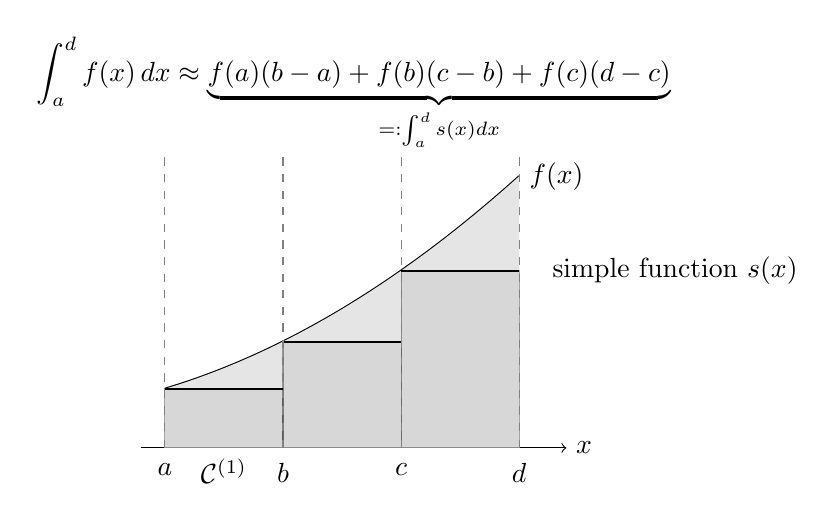
\begin{tikzpicture}[scale=1.5]
  			
  			\draw[->] (-0.2,0) -- (3.4,0) node[right] {$x$};
 			
  			
  			\draw[thick,domain=0:3,smooth] plot(\x,{0.5+0.3*\x+0.1*\x*\x}) node[right] {$f(x)$};
  			
  			\fill[gray!20] (0,0) -- plot[domain=0:3] (\x,{0.5+0.3*\x+0.1*\x*\x}) -- (3,0) -- cycle;
  			
  			\draw[fill=gray!50,opacity=0.35] (0,0) rectangle (1,0.5);
  			\node at (0.5,-0.2) {$\mathcal{C}^{(1)}$}; 
  			\draw[fill=gray!50,opacity=0.35] (1,0) rectangle (2,0.9);
  			\draw[fill=gray!50,opacity=0.35] (2,0) rectangle (3,1.5);
  			
  			\draw[thick] (0,0.5)--(1,0.5);
  			\draw[thick] (1,0.9)--(2,0.9);
  			\draw[thick] (2,1.5)--(3,1.5);
 	 		\node[above left] at (0.8,0.5) {};
  			
  			\foreach \x in {0,1,2,3} \draw[dashed,gray] (\x,0) -- (\x,2.5);
  			
  			\node[anchor=north] at (0,-0.05) {$a$};
  			\node[anchor=north] at (1,-0.05) {$b$};
  			\node[anchor=north] at (2,-0.05) {$c$};
  			\node[anchor=north] at (3,-0.05) {$d$};
  			\node at (1.6,3.0) {$\displaystyle \int_a^d f(x)\,dx \approx \underbrace{f(a)(b-a) + f(b)(c-b)+f(c)(d-c)}_{=:\int_a^d s(x)dx}$};
  			\node [anchor=west] at (3.2,1.5) {simple function $s(x)$};
			\end{tikzpicture}
		\end{figure}
 		It is useful to think of the Lebesgue integral as a function that maps 
 		an integrable function $f$ to the value of its integral, 
		$$ f \mapsto \int_{{\bf x}} f({\bf x}) d{\bf x}.$$ 
		The precise definition of this function, whose domain 
		consists of the integrable functions, is a cornerstone of 
		measure theory \cite[Ch. 1]{RudinBook}.
					\\ 
		See also: function.},
	first={Lebesgue integral},
	text={Lebesgue integral},
	type=math, 
	plural={Lebesgue integrals},
	firstplural={Lebesgue integrals}
}

\newglossaryentry{conditionalexpect}
{name={conditional expectation}, 
	description={Consider a numeric random variable (RV) ${\bf x}\in \mathbb{R}^{d}$ defined on a 
                 probability space $\mathcal{P}=(\Omega,\mathcal{F},\mathbb{P})$. 
                 Let $\Sigma' \subseteq \Sigma$ be a (sub-) $\sigma$-algebra that 
                  represents partial information about the outcome of a random experiment. 
                  The conditional expectation\index{conditional expectation} of 
                  ${\bf x}$ given (or conditioned on) $\Sigma'$, denoted 
                  $\mathbb{E} \{ {\bf x}\mid \Sigma'\}$, is a numeric random variable (RV) 
				  that \cite{BillingsleyProbMeasure,durrett2010probability}
                  \begin{itemize}
                   \item is measurable with respect to $\Sigma'$, and
                    \item satisfies
			  		$$
    		  		\int_{\mathcal{A}} \mathbb{E} \{{\bf x}\mid \Sigma'\} {\rm d} \mathbb{P}=
    		  		\int_{\mathcal{A}} {\bf x}{\rm d} \mathbb{P}\quad \text{for any } \mathcal{A} \in \Sigma'.
			  		$$
                \end{itemize}
               Intuitively, $\mathbb{E} \{{\bf x}\mid \mathcal{F}'\}$ summarizes 
               the average value of ${\bf x}$ using only information contained 
               in the (typically smaller) $\sigma$-algebra $\Sigma'$ 
			   \cite{BillingsleyProbMeasure,GrayProbBook,ross2013first}. \\
              See also: expectation, $\sigma$-algebra, probability space.}, 
 	first={conditional expectation},
 	plural={conditional expectations}, 
 	type=math, 
 	firstplural={conditional expectations},  
 	text={conditional expectation}
}

\newglossaryentry{conditionalpmf}
{name={conditional probability mass function (conditional pmf)}, 
	description={Consider two discrete random variables (discrete RVs) $y$ and $x$ defined on 
                  the same probability space $(\Omega,\mathcal{F},\mathbb{P}\left(\cdot\right))$. 
                  The conditional pmf\index{conditional pmf} of $y$ given 
				  (or conditioned on) $x$ is denoted 
                $p^{(y\mid x)}\left(\cdot \mid \cdot\right)$ and is defined by
                \[
                  p^{(y\mid x)}\left(y' \mid x'\right)
                  :=
                  \mathbb{P}\left(y=y' \mid x=x'\right),
               \]
                for all realizations $y',x'$ with 
                $\mathbb{P}\left(x=x'\right)>0$. 
                Equivalently, the conditional pmf can be expressed using 
                conditional expectation as
                \[
                  p^{(y\mid x)}\left(y' \mid x'\right)
                  =
                  \mathbb{E} \{\mathbb{I}_{y=y'}\mid \Sigma(x)\}(x'),
                \]
                where $\Sigma(x)$ denotes the $\sigma$-algebra generated by 
                 the random variable (RV) $x$. \\
              See also: conditional expectation, probability mass function (pmf), probability space.}, 
 	first={conditional probability mass function (conditional pmf)},
 	firstplural={conditional probability mass functoins (conditional pmfs)}, 
 	type=math, 
 	plural={conditional pmfs},  
 	text={conditional pmf}
}


\newglossaryentry{iid}
{name={independent and identically distributed (i.i.d.)}, 
	description={A collection of random variables (RVs)\linebreak ${\bf z}^{(1)}, \,\ldots, \,{\bf z}^{(m)}$ is 
		referred to as i.i.d.\index{independent and identically distributed (i.i.d.)} 
		if each ${\bf z}^{(r)}$ follows the same probability distribution, and 
		the random variables (RVs) are mutually independent. That is, for any collection of 
		events $\mathcal{A}_1, \,\ldots, \,\mathcal{A}_m$, we have
       		\[
          		\mathbb{P}\left( {\bf z}^{(1)} \in \mathcal{A}_1, \,\ldots, \,{\bf z}^{(m)} \in \mathcal{A}_{m}\right) 
         		= \prod_{r=1}^{m} \mathbb{P}\left( {\bf z}^{(r)} \in \mathcal{A}_r\right).
         	\]
				\\
		See also: random variable (RV), probability distribution, event, data point, independent and identically distributed assumption (i.i.d.\ assumption).},
	first={independent and identically distributed (i.i.d.)},
	type=math, 
	text={{i.i.d.}} 
}

\newglossaryentry{preimage}
{name={preimage}, 
	description={Consider a function\index{preimage} $f\colon \mathcal{U} \rightarrow \mathcal{V}$ 
		between two sets. The preimage $f^{-1}(\mathcal{B})$ of a subset $\mathcal{B} \subseteq \mathcal{V}$ is the set 
		of all inputs $u \in \mathcal{U}$ that are mapped into $\mathcal{B}$ by $f$, i.e.,
		\[
		f^{-1}(\mathcal{B}) :=\{ u \in \mathcal{U} \mid f(u) \in \mathcal{B} \}.
		\]
		The preimage is well defined even if the function $f$ is non-invertible \cite{RudinBookPrinciplesMatheAnalysis}.
		\\
		See also: function. },
	first={preimage},
	type=math, 
	text={preimage}
}

\newglossaryentry{measurable}
{name={measurable}, 
	description={Consider\index{measurable} a random experiment, such as recording 
		the air temperature at an Finnish Meteorological Institute (FMI) weather station. The corresponding sample space 
		$\Omega$ consists of all possible outcomes $\omega$ (e.g., 
		all possible temperature values in degree Celsius). In many machine learning (ML) 
		applications, we are not interested in the exact outcome $\omega$, but only 
		whether it belongs to a subset $\mathcal{A} \subseteq \Omega$ 
		(e.g., determining whether the temperature is below zero degrees). 
		We call such a subset $\mathcal{A}$ measurable if it is possible to 
		decide, for any outcome $\omega$, whether $\omega\in \mathcal{A}$ 
		or not (see Fig.\ \ref{fig_measurable_dict}). \\
		\begin{figure}[H]
		\begin{center}
		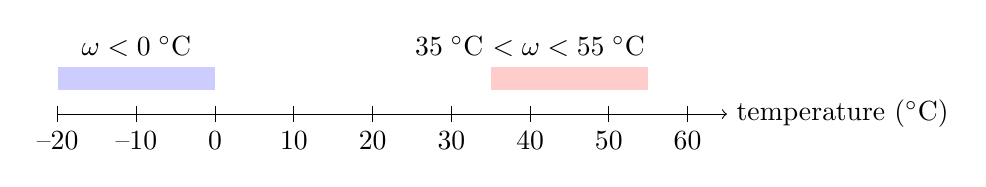
\begin{tikzpicture}
			
			\draw[->] (0,0) -- (8.5,0) node[right] {temperature ($^\circ$C)};
			
			\foreach \x/\label in {0/--20, 1/--10, 2/0, 3/10, 4/20, 5/30, 6/40, 7/50, 8/60} {
				\draw (\x,0.1) -- (\x,-0.1);
				\node[below] at (\x,-0.1) {\label};
			}
			
			\fill[blue!20] (0,0.3) rectangle (2,0.6);
			\node[above] at (1,0.6) {$\omega< 0\;^\circ$C};
			
			\fill[red!20] (5.5,0.3) rectangle (7.5,0.6);
			\node[above] at (6,0.6) {$35\;^\circ$C $< \omega< 55\;^\circ$C};
			\vspace*{10mm}
			\end{tikzpicture}
			\vspace*{10mm}
			\end{center}
			\caption{A sample space constituted by all possible temperature values $\omega$ 
			that can occur at an Finnish Meteorological Institute (FMI) station. Two measurable subsets of temperature 
			values, denoted by $\mathcal{A}^{(1)}$ and $\mathcal{A}^{(2)}$, are highlighted. For any 
			actual temperature value $\omega$, it is possible to determine (via some equipment) 
			whether $\omega\in \mathcal{A}^{(1)}$ and whether $\omega\in \mathcal{A}^{(2)}$. 
			\label{fig_measurable_dict}} 
		\end{figure}
		In principle, measurable sets could be chosen freely (e.g., depending on the resolution of the 
		measuring equipment). However, it is often useful to impose certain completeness requirements 
		on the collection of measurable sets. For example, the sample space itself should be 
		measurable, and the union of two measurable sets should also be measurable. These completeness 
		requirements can be formalized via the concept of a $\sigma$-algebra (or $\sigma$-field) 
		\cite{RudinBook}, \cite{BillingsleyProbMeasure}, \cite{durrett2010probability}. 
		A measurable space is a pair $\big(\mathcal{X},\mathcal{F}\big)$ that consists of an arbitrary 
		set $\mathcal{X}$ and a collection $\mathcal{F}$ of measurable subsets of $\mathcal{X}$ 
		that form a $\sigma$-algebra. 
		\\
		See also: sample space, $\sigma$-algebra, probability.},
	first={measurable},
	type=math, 
	text={measurable} 
}

\newglossaryentry{sigmaalgebra}
{name={$\sigma$-algebra}, 
sort={sigma-algebra},
	description={Consider a random experiment with a sample space $\Omega$. 
		A $\sigma$-algebra\index{$\sigma$-algebra} (or $\sigma$-field) $\Sigma$ 
		is a collection of subsets of $\Omega$ with the following properties 
		\cite{RudinBook}, \cite{BillingsleyProbMeasure}, \cite{durrett2010probability}:
		 \begin{itemize}
		 	\item The empty set $\emptyset$ and the entire sample space 
		 	$\Omega$ belong to $\Sigma$, i.e., $\emptyset \in \Sigma$ and $\Omega\in \Sigma$.
		 	\item If a set $\mathcal{A}$ belongs to $\Sigma$, then its complement 
		 	$\Omega\setminus \mathcal{A}$ also belongs to $\Sigma$, i.e., 
		 	$\mathcal{A} \in \Sigma$ implies $\Omega\setminus \mathcal{A} \in \Sigma$.
		 	\item If a countable collection of sets $\mathcal{A}_1, \,\mathcal{A}_2, \,\ldots$ belongs 
			to $\Sigma$, 
		 	then their union also belongs to $\Sigma$, i.e.,
		 	$\mathcal{A}_1, \,\mathcal{A}_2, \,\ldots \in \Sigma$ implies 
		 	$\bigcup_{i=1}^{\infty} \mathcal{A}_i \in \Sigma$.	
		 \end{itemize}			 
		See also: sample space, random variable (RV), probability space.},
	first={$\sigma$-algebra},
	type=math, 
	text={$\sigma$-algebra} 
}

\newglossaryentry{sigmafield}
{name={$\sigma$-field}, 
sort={sigma-field},
	description={See $\sigma$-algebra\index{$\sigma$-field}.}, 
	first={$\sigma$-field},
	type=math,
	text={$\sigma$-field} 
}

\newglossaryentry{injective}
{name={injective}, 
	description={A function $f: \mathcal{U} \rightarrow \mathcal{V}$ is injective\index{injective} 
		if it maps distinct elements of its domain to distinct elements 
		of its co-domain, 
    		i.e., if $f(u_1) = f(u_2)$ implies $u_1 = u_2$ for all $u_1, u_2 \in \mathcal{U}$ 
        		\cite{HalmosSet}. 
    		Equivalently, no two different function inputs are mapped to the same function output.
				\\
		See also: function.},
	first={injective},
	type=math,
	text={injective} 
}


\newglossaryentry{typicalset}
{name={typical set}, 
	description={See probability mass function (pmf)\index{typical set}.}, 
 	first={typical set},
 	firstplural={typical sets},
 	type=math,
 	plural={typical sets},
 	text={typical set} 
}